
% Template for Elsevier CRC journal article
% version 1.1 dated 16 March 2010

% This file (c) 2010 Elsevier Ltd.  Modifications may be freely made,
% provided the edited file is saved under a different name

% This file contains modifications for Procedia Computer Science
% but may easily be adapted to other journals

% Changes since version 1.0
% - elsarticle class option changed from 1p to 3p (to better reflect CRC layout)

%-----------------------------------------------------------------------------------

%% This template uses the elsarticle.cls document class and the extension package ecrc.sty
%% For full documentation on usage of elsarticle.cls, consult the documentation "elsdoc.pdf"
%% Further resources available at http://www.elsevier.com/latex

%-----------------------------------------------------------------------------------

%%%%%%%%%%%%%%%%%%%%%%%%%%%%%%%%%%%%%%%%%%%%%%
%%%%%%%%%%%%%%%%%%%%%%%%%%%%%%%%%%%%%%%%%%%%%%
%%                                          %%
%% Important note on usage                  %%
%% -----------------------                  %%
%% This file must be compiled with PDFLaTeX %%
%% Using standard LaTeX will not work!      %%
%%                                          %%
%%%%%%%%%%%%%%%%%%%%%%%%%%%%%%%%%%%%%%%%%%%%%%
%%%%%%%%%%%%%%%%%%%%%%%%%%%%%%%%%%%%%%%%%%%%%%

%% The '3p' and 'times' class options of elsarticle are used for Elsevier CRC
\documentclass[3p,times]{elsarticle} %this is original one for 1 column
%\documentclass[5p,times,twocolumn]{elsarticle}

%% The `ecrc' package must be called to make the CRC functionality available
%\usepackage{ecrc}

%% The ecrc package defines commands needed for running heads and logos.
%% For running heads, you can set the journal name, the volume, the starting page and the authors

%% set the volume if you know. Otherwise `00'
%\volume{00}

%% set the starting page if not 1
%\firstpage{1}

%% Give the name of the journal
%\journalname{Procedia Computer Science}

%% Give the author list to appear in the running head
%% Example \runauth{C.V. Radhakrishnan et al.}
%\runauth{M. Z. Alam et al.}

%% The choice of journal logo is determined by the \jid and \jnltitlelogo commands.
%% A user-supplied logo with the name <\jid>logo.pdf will be inserted if present.
%% e.g. if \jid{yspmi} the system will look for a file yspmilogo.pdf
%% Otherwise the content of \jnltitlelogo will be set between horizontal lines as a default logo

%% Give the abbreviation of the Journal.
%\jid{procs}

%% Give a short journal name for the dummy logo (if needed)
%\jnltitlelogo{Procedia Computer Science}

%% Hereafter the template follows `elsarticle'.
%% For more details see the existing template files elsarticle-template-harv.tex and elsarticle-template-num.tex.

%% Elsevier CRC generally uses a numbered reference style
%% For this, the conventions of elsarticle-template-num.tex should be followed (included below)
%% If using TeX, use the style file elsarticle-num.bst

%% End of ecrc-specific commands
%%%%%%%%%%%%%%%%%%%%%%%%%%%%%%%%%%%%%%%%%%%%%%%%%%%%%%%%%%%%%%%%%%%%%%%%%%

%% The amssymb package provides various useful mathematical symbols
\usepackage{amssymb}
%% The amsthm package provides extended theorem environments
\usepackage{amsthm}
\usepackage{amsmath}

%% The lineno packages adds line numbers. Start line numbering with
%% \begin{linenumbers}, end it with \end{linenumbers}. Or switch it on
%% for the whole article with \linenumbers after \end{frontmatter}.
\usepackage{lineno}

%% natbib.sty is loaded by default. However, natbib options can be
%% provided with \biboptions{...} command. Following options are
%% valid:

%%   round  -  round parentheses are used (default)
%%   square -  square brackets are used   [option]
%%   curly  -  curly braces are used      {option}
%%   angle  -  angle brackets are used    <option>
%%   semicolon  -  multiple citations separated by semi-colon
%%   colon  - same as semicolon, an earlier confusion
%%   comma  -  separated by comma
%%   numbers-  selects numerical citations
%%   super  -  numerical citations as superscripts
%%   sort   -  sorts multiple citations according to order in ref. list
%%   sort&compress   -  like sort, but also compresses numerical citations
%%   compress - compresses without sorting
%%
%% \biboptions{comma,round}

% \biboptions{}

% if you have landscape tables
\usepackage[figuresright]{rotating}

% put your own definitions here:
%   \newcommand{\cZ}{\cal{Z}}
%   \newtheorem{def}{Definition}[section]
%   ...

\usepackage{hyperref}
\usepackage{multirow}
\usepackage{color}
\usepackage{xcolor-patch}
\usepackage{setspace}
\doublespacing

% *** SPECIALIZED LIST PACKAGES ***
%
\usepackage{algorithmic, algorithm}
% algorithmic.sty was written by Peter Williams and Rogerio Brito.
% This package provides an algorithmic environment fo describing algorithms.
% You can use the algorithmic environment in-text or within a figure
% environment to provide for a floating algorithm. Do NOT use the algorithm
% floating environment provided by algorithm.sty (by the same authors) or
% algorithm2e.sty (by Christophe Fiorio) as the IEEE does not use dedicated
% algorithm float types and packages that provide these will not provide
% correct IEEE style captions. The latest version and documentation of
% algorithmic.sty can be obtained at:
% http://www.ctan.org/pkg/algorithms
% Also of interest may be the (relatively newer and more customizable)
% algorithmicx.sty package by Szasz Janos:
% http://www.ctan.org/pkg/algorithmicx

% *** PDF, URL AND HYPERLINK PACKAGES ***
%
\usepackage{url}
% url.sty was written by Donald Arseneau. It provides better support for
% handling and breaking URLs. url.sty is already installed on most LaTeX
% systems. The latest version and documentation can be obtained at:
% http://www.ctan.org/pkg/url
% Basically, \url{my_url_here}.

% add words to TeX's hyphenation exception list
%\hyphenation{author another created financial paper re-commend-ed Post-Script}

% correct bad hyphenation here
\hyphenation{op-tical net-works semi-conduc-tor}

% declarations for front matter

%\doublespace
\begin{document}
	
	\begin{frontmatter}
		
		%% Title, authors and addresses
		
		%% use the tnoteref command within \title for footnotes;
		%% use the tnotetext command for the associated footnote;
		%% use the fnref command within \author or \address for footnotes;
		%% use the fntext command for the associated footnote;
		%% use the corref command within \author for corresponding author footnotes;
		%% use the cortext command for the associated footnote;
		%% use the ead command for the email address,
		%% and the form \ead[url] for the home page:
		%%
		%% \title{Title\tnoteref{label1}}
		%% \tnotetext[label1]{}
		%% \author{Name\corref{cor1}\fnref{label2}}
		%% \ead{email address}
		%% \ead[url]{home page}
		%% \fntext[label2]{}
		%% \cortext[cor1]{}
		%% \address{Address\fnref{label3}}
		%% \fntext[label3]{}
		
		%\dochead{}
		%% Use \dochead if there is an article header, e.g. \dochead{Short communication}
		
		\title{Feature Ranking based Ensemble Classifiers for survivability prediction of ICU patients using Lab Test data}
		%\tnotetext[mytitlenote]{Full document is available in on\href{http://www.ctan.org/tex-archive/macros/latex/contrib/elsarticle}.}
		
		%% use optional labels to link authors explicitly to addresses:
		%% \author[label1,label2]{<author name>}
		%% \address[label1]{<address>}
		%% \address[label2]{<address>}
		
		%% Group authors per affiliation:
		%% include affiliations in footnotes:
		\author[buetaddress]{Md. Zahangir Alam\fnref{myfootnote}}
		\ead{zahangirbd@gmail.com}
		
		\author[uaeuaddress]{Mohammad M. Masud \corref{mycorrespondingauthor}}
		\ead{m.masud@uaeu.ac.ae}
        
        \author[buetaddress]{M. Saifur Rahman}
		\ead{mrahman@cse.buet.ac.bd}
		
		\author[uaeuaddress]{Muhsin Cheratta}
		\ead{muhsin.j@uaeu.ac.ae}
		
		\author[buetaddress]{Muhammad Ali Nayeem\fnref{myfootnote}}			
		\ead{ali\_nayeem@cse.buet.ac.bd}			
					
		\author[buetaddress]{M. Sohel Rahman}
        \cortext[mycorrespondingauthor]{Corresponding author. E-mail: \url{m.masud@uaeu.ac.ae}}		
        \ead{msrahman@cse.buet.ac.bd}
		
		%\address[buetaddress]{Department of Computer Science and Engineering (CSE), ECE Building, West Palashi, Bangladesh University of Engineering and Technology (BUET), Dhaka-1000, Bangladesh.}
		
		\address[buetaddress]{Department of CSE, BUET, ECE Building, West Palasi, Dhaka-1205, Bangladesh.}
		\address[uaeuaddress]{College of Information Technology, United Arab Emirates University, Al Ain, UAE.}
		\fntext[myfootnote]{Supported by an ICT (PhD) Fellowship}
		
		\begin{abstract}
			Clinical decision support systems (CDSS) are getting significant attention in recent years for their role and impact on the improvement in quality, safety, efficiency, and effectiveness in the context of healthcare. Advanced data analytics enabled CDSS are found to perform more accurately and timely than traditional systems. In this domain, survival prediction or deterioration prediction of critical cared patients, such as intensive care unit (ICU) patients, is an active research area. Early deterioration prediction can help health care providers to take proper and timely actions for the patients. The research works in this area are mostly based on the vital signs. Very few studies are available on survival prediction using lab tests data. Although some research works have made some advancement in this area, the accuracy is still suffering and is not satisfactory. \textcolor{blue}{Hence, the main goal of the current research work is to provide a technique to improve the accuracy and efficiency of survival prediction using lab test data.} We propose a feature ranking based ensemble of classifiers for survival prediction of ICU patients using lab test data. In the proposed approach, features are evaluated first and subsets of `useful' features are selected. Subsequently, training data with the selected features are clustered using a novel feature vector compaction (FVC) technique. Finally, ensemble classifier models are trained. Extensive experiments in more than 3000 different settings on 6 datasets of ICU patients have been conducted to evaluate the efficacy of our approach. The experimental results demonstrate that this technique outperforms other approaches. 
		\end{abstract}
		
		\begin{keyword}
			%% keywords here, in the form: keyword \sep keyword
			
			%% MSC codes here, in the form: \MSC code \sep code
			%% or \MSC[2008] code \sep code (2000 is the default)
			
			%%\texttt{elsarticle.cls}\sep \LaTeX\sep Elsevier \sep template
			%%\MSC[2010] 00-01\sep  99-00
			
			ICU Patients\sep Mortality Prediction\sep  Feature Ranking \sep Feature Vector Compaction\sep  Feature Grouping\sep  Lab Test Data\sep Clinical Prediction\sep Clustering \sep Clinical decision support
			
		\end{keyword}
		
	\end{frontmatter}
	
	%%
	%% Start line numbering here if you want
	%%
	% \linenumbers
	
	%% main text
	
    \section{Introduction}
Research on clinical decision support (CDS) and clinical prediction (CP) has been getting high attention in recent years for its significant impacts on the improvements in quality, safety, efficiency, and effectiveness in health-care domain. In reality, for some cases, patients are intensively cared and monitored by the health care providers, such as, intensive care unit (ICU) patients. Timely and effective actions recommended by CDS or CP can help care-givers to take necessary actions to avoid any unwanted circumstances or to make an improvement in health condition. Therefore, study in this domain has been gaining more and more emphasis by the researchers since the last decade.

Nowadays most of the hospitals, clinics and health institutions are deployed with various electronic health monitoring devices which are continuously producing data. Many of these medical facilities store these data in  a systematic and standard manner in the form of Electronic Health Records (EHRs). Researchers have already demonstrated much advancement on data analytics techniques. These advanced techniques, applied on EHRs, can create great improvement in CDS and CP systems with the help of high performance computing services.

Health data of our interest could be continuous, such as, vital signs or they could be discrete or incremental, such as, lab tests data. Moreover, there are other types of data available additionally, such as, records of medication, nurse notes, demographic data, administrative (e.g. admissions) and procedural (e.g. caregiver name) information. \textcolor{blue}{Among these, vital signs and lab test records have mostly been used in the literature \cite{Mao,Fialho,Baumgartner,Cheng, Ghassemi2015, Jin2018, Yoon2016, Johnson2017, Calvert2016, Suresh2017, Bhattacharya2017, Xie2017, Awad2017, Nguyen2017, Zhang2017, Johnson2nd2017, Davoodi2018, Sadeghi2018, Zheng2018, Johnson3rd2018, Zahid2018, Purushotham2018, Meyer2018, Hsieh2018, Ho2019, Gennatas2019, Torres2019}}. Using the vital signs data, some studies have illustrated the possibility to predict patient situation (e.g., deterioration) ahead of time with a goal to warn caregivers to take timely and reliable measures to save the patient’s life. Many challenges are involved in building such a system using vital signs \textcolor{blue}{as discussed in \cite{Mao,Fialho,Baumgartner,Cheng, ZhengpingChe2016, Zahid2018, Zheng2018, Xiao2018}. On the other hand, research works are relatively rare focused on lab test data. To the best of our knowledge the only work in the literature considering only lab test data are the work of  Masud \& Harahsheh \cite{mehedy-masud:2017:fvc} and Masud and Cheratta \cite{mehedy-masud:2018:frmwrk}. Hence, this study primarily focuses on lab test records}.

The lab test records are not readily usable for building a good prediction system. It contains severe challenges related to be treated as a feature. Some of these challenges are mentioned in some recent studies \cite{mehedy-masud:2017:fvc, mehedy-masud:2018:frmwrk} and are discussed as follows for the sake of completeness. The first challenge is a variable length feature vector. It occurs because each patient undergoes a different subsets (possibly overlapping) of lab tests. As a result, there is no uniform feature vector across all patients. But most learning algorithms need uniform feature vectors, which necessitates the prediction of missing values into the feature vector of each patient. The second challenge is the high dimensionality of the data due to the large number different possible lab tests that can be done on a patient. The third challenge is the class imbalance, which is also found in many problems in the medical domain. And the last but not the least challenge is the longitudinal features, i.e., a patient may undergo the same test more than once. Interestingly, the first two challenges are interrelated making the scenario more complex. For example, missing values are introduced primarily because of high dimensionality, and they bring noise, redundancy, and sparsity in the dataset. One of the general solutions in this context is to apply some kind of feature selection: features may be evaluated and examined by some standard feature ranking algorithms that give score to each feature. Clearly missing values pose an issue in this approach and need be handled properly. Additionally, class imbalance make the situation worse. In \cite{mehedy-masud:2017:fvc, mehedy-masud:2018:frmwrk}, a subset of the authors proposed a novel feature vector compaction (FVC) technique for addressing the missing values and high dimensionality problem and presented some preliminary results. The current work proposes several modifications to FVC in order to improve its efficiency and effectiveness.

The feature vector compaction (FVC) exploits a measure called vacuum count (VC). It deals with missing values found when two feature vectors are combined. In this work we consider another angle as follows. Instead of only focusing on missing values, we also focus on how many common features are available between two sets of feature vectors. Thus, we propose a new measure called common feature count (CFC) to compare two sets of feature vectors.

The main contributions of this research work are as follows. At first we propose a feature ranking based feature selection approach along with FVC technique for lab test results with a goal to improve the performance of the clinical prediction. Secondly, the proposed methodology systematically handles the missing data, high dimension, and class imbalance issues. Thirdly we explore how the proposed CFC technique can be used to improve the accuracy of the mortality prediction. And, last but not the least, we propose an ensemble approach to achieve even better results.

This paper is organized as follows. Section \ref{s:related} presents a brief literature review. Section \ref{s:methods} describes the proposed techniques in detail. Then Section \ref{s:experiments} states the experimental setup and other information related thereof. Section \ref{s:results} presents the results of the experiments over various datasets with an in-depth analysis followed by a discussion in Section \ref{s:discussions}. Finally Section \ref{s:conclusion} briefly concludes the paper with future research directions.

	\section{Related works} \label{s:related}
\textcolor{blue}{ In this section, we briefly discuss several recent studies on the mortality prediction of ICU patients and analyze their main differences from that approach that we adopted in this study. We provided a more comprehensive review for the interested readers in the supplementary materials.}

\textcolor{blue}{Calvert \textit{et al.} developed an algorithm, namely, \textit{AutoTriage}, which uses eight common clinical variables, mostly from physiological measurements, and 2/3 discretized variables \cite{Calvert2016}. These clinical variables produce sub-scores. A combination of weighted sub-scores is used as the final score for the mortality prediction of ICU patients. They conducted experiments on MIMIC-III (Medical Information Mart for Intensive Care III) hospital database of ICU patients. Bhattacharya \textit{et al.} conducted a study for ICU mortality prediction addressing the class imbalance issue of the ICU data in the context of binary classification through a feature transformation approach \cite{Bhattacharya2017}. They used demographic data, 37 lab investigations and some physiological signal measurements for their experiments. Xie \textit{et al.} outlined the essential procedures and concepts for developing prediction models for in-hospital mortality prediction for ICU patients in \cite{Xie2017}. In their work, Artificial Neural Network (ANN), Decision Tree (DT), and Support Vector Machines (SVM) exhibited promising results in analyzing large and heterogeneous data compared to Logistic Regression (LR). They used physiological variables along with others. Awad \textit{et al.} proposed a method called Early Mortality Prediction for ICU patients (EMPICU) \cite{Awad2017} to predict mortality after six hours from admission to ICU. They included demographic, physiological, vital signs as well as laboratory test variables collected from the MIMIC-II database. Nguyen \textit{et al.} proposed a deep learning architecture based on Long Short-Term Memory networks (LSTM) with layered attentions mechanism to predict ICU mortality to address the issue of missing measurements \cite{Nguyen2017}. They used 41 measure types including vital signs.} 

\textcolor{blue}{In an attempt to present benchmarks, Johnson \textit{et al.} conducted 38 experiments of 28 published studies that used the MIMIC database to reproduce the cohorts (i.e., a group of variables) used in these studies in the context of the performance of mortality prediction models \cite{Johnson2nd2017}. Darabi \textit{et al.} developed a technique in which they applied Gradient Boosting Decision Trees (GBT) and deep neural networks to predict the mortality of ICU patients \cite{Darabi2018}. They used grid-search to find the optimal parameters for the model. They conducted their experiments on the medical codes (diagnosis codes, procedure codes, diagnosis-related group code) collected from the MIMIC-III database.} 

\textcolor{blue}{Sadeghia \textit{et al.} proposed a method which utilized statistical and signal-based features for early hospital mortality prediction \cite{Sadeghi2018}. They used only vital signals, i.e., heart signals of the patients and these were collected from the MIMIC-III database. Zheng and Shi utilized LSTM and Recurrent Neural Network (RNN) based deep learning techniques for ICU mortality prediction \cite{Zheng2018}. They used a statistical approach to preprocess the data. They presented a data imputation method based on the Gaussian process. They used ICU data containing 36 variables from the PhysioNet. These 36 features are mentioned in terms of importance from a medical perspective.} 

\textcolor{blue}{Zahid and Joon Lee explored deep learning techniques focusing on the Self Normalizing Neural network (SNN) for predicting mortality of the ICU patients \cite{Zahid2018}. They used demographic information, vital physiological signs, progress notes by physicians and nurses, reports from imaging studies, lab test results, International Classification of Diseases-9 (ICD-9) codes, daily Simplified Acute Physiology Score (SAPS) and Sequential Organ Failure Assessment (SOFA) score, discharge summaries, hospital lengths of stay (LoS), and output of the hospital mortality. Purushotham \textit{et al.} performed a study for presenting benchmark results for clinical prediction tasks (e.g., mortality prediction, LoS prediction, and ICD-9 code group prediction) using deep learning models, Super ICU Learner Algorithm (SICULA), and SAPS-II and SOFA \cite{Purushotham2018}. They found the deep learning models performing consistently better than all other approaches.} 

\textcolor{blue}{Gennatas \textit{et al.} have proposed Expert-Augmented Machine Learning (EAML) that guides the extraction of expert knowledge and it's integration into machine learning models \cite{Gennatas2019}. They conducted experiments on MIMIC-II \& MIMIC-III datasets for predicting mortality of the ICU patients. They used vital signs along with other clinical variables in their experiments. Caicedo-Torres and Gutierrez proposed a deep multi-scale convolutional architecture trained on the MIMIC-III dataset for predicting mortality of ICU patients \cite{Torres2019}. They demonstrated visual explanations focusing on how the network treats these inputs as important features. They used 22 different variables including vital signs which are somewhat similar to the concepts used by the SAPS-II score. De Lange \textit{et al.} proposed a cumulative prognostic score model for predicting mortality of ICU patients who are older than 80 years \cite{Lange2019}. They developed a multi-variable LR model in which variables are selected using LASSO. Data of 306 ICU patient from 24 European countries were collected and their 24 clinical variables were used in the experiment.} Herland \textit{et al.} have conducted a comprehensive survey on clinical data mining applications based on big data in health informatics \cite{Herland}. Cai \textit{et al.}  proposed an approach based on the Bayesian network to develop models using EHRs for real-time prediction of several targets, including the length of hospital stay, mortality, and readmission of hospitalized patients \cite{Cai:2016}.

Now we analyze how our study is fundamentally different from the research endeavors mentioned above. To predict the survival of ICU patients, most of the above studies used vital signs or demographic variables and some focused mainly on clinical notes, whereas we only used lab test results in our approach. Some works indeed consider lab tests measurements albeit only a small set thereof and that too in combination with other features. On the contrary, we consider only lab tests measurements and a large set thereof. Next, we find the majority of the above studies focusing on a single machine learning/data mining technique. However, our work proposes a hybrid approach: features are selected at first and then ensemble models are generated using the FVC technique with various ensemble classification techniques. Therefore we believe that our current approach applies to any CDS related systems in general. Besides, a great advantage of our FVC based approach, compared to any machine learning technique, is its inherent capability of tackling the curse of dimensionality\cite{Meyer2018} of hospital database Big data. Furthermore, some of the previous studies deal with particular disease-oriented data. But we generally work for the mortality of ICU patients irrespective of any disease. Also, we have used different kinds of datasets for the experiments. More will be elaborated at later sections of this paper.


%\textcolor{blue}{Additionally, some of the above deep learning methodology based studies deal with Big data in the context of in-hospital mortality of ICU patients. According to Meyer \textit{et al.} \cite{Meyer2018} adding more variables into the actual data matrix increases the dimension of the matrix which may become computationally burdensome for this kind of model. But FVC technique \cite{mehedy-masud:2017:fvc} is reverse of this, deals with large data and has shown the improved performance on training or testing time.}

Finally, we would like to mention that, a subset of the authors were involved in proposing the FVC approach in \cite{mehedy-masud:2017:fvc} and ORCU (a novel orthogonal clustering technique) in \cite{mehedy-masud:2018:frmwrk} where some preliminary experiments and findings were discussed. In this study, we proposed further improvements  \cite{mehedy-masud:2017:fvc,mehedy-masud:2018:frmwrk} and conducted extensive experiments with real clinical data thereby reaching a promising milestone in this research endeavor.
    \section{Proposed approach} \label{s:methods}

\subsection{Datasets} \label{sec:datapreparation}
The datasets used in this study are MIMIC II (Physionet MIMICII) \cite{MIMIC2} and MIMIC III (Physionet-MIMICIII) \cite{MIMIC3}. These databases are developed by the Multi-parameter Intelligent Monitoring in Intensive Care (MIMIC) project at the Laboratory of Computational Physiology at MIT, funded by the National Institute of Biomedical Imaging and Bioengineering. For each dataset the data holds the results of lab tests produced through each test done on each patient. Each lab test result contains the numeric value of the lab test performed, a flag (binary) indicating whether the result is ``normal'' or ``abnormal'', the unit of measurement, and date/time of the test performed. 

\subsubsection{MIMIC II} \label{sec:MIMIC2}
MIMIC II data were collected between 2001 and 2008 from a variety of ICUs. MIMIC II database contains the records of 33,000 patients of which around 25,000 are adults (having age $\geq$ 15 years at time of last admission) and near about 8000 are neonates (age $\leq$ 1 month at the time of first admission). These patients were admitted into over 36,000 hospitals and stayed in over 40,000 ICUs. MIMIC II consists of two major components: clinical data and physiological waveforms. The clinical data are used in this study.   

This clinical dataset consists 40 different tables, each containing different types of information, such  as, demographic data (available in \textit{General} category), hospital admission data, ICU stay data, medication information, lab test results (available in \textit{Labtests}), nurse notes and so on. Among these tables, only the lab test data is used in this work to investigate the effectiveness thereof in predicting mortality. In addition to the lab test results, the patient's final status, i.e., whether the patient survived or died in the ICU is used. 

\subsubsection{MIMIC III} \label{sec:MIMIC3}
MIMIC III data were collected between 2001 to 2012 from more than 50,000 hospital admissions. This database comprises 25 different tables, each holding different types of information, for example, demographic data, hospital admission data, ICU stay data, medication information, lab test results, nurse notes and so on. The lab test data (called \textit{Labevents}) as well as some demographic and admission related information from among these tables are used primarily in our study.

The \textit{Patient} table, which contains the date of birth, gender, and whether the patient survived or died is used in this work. The \textit{Admissions} table, which holds the date of admission, date of discharge, ethnicity, and diagnosis of the patient is also used here. The patient's age is computed by joining the \textit{Patient} table and \textit{Admissions} table and they by deducting the date of birth from the date of admission. Finally, the \textit{ICUStays} table, that contains the length of stay of the patient, is used in this study.

\subsubsection{Feature extraction and vector generation} 
\textcolor{blue}{At first, we make a profile for each patient based on his/her age as has been done in \cite{mehedy-masud:2017:fvc} and form four different groups: Newborn, Infant, Child, Adult, and Senior. Table \ref{t:groupbyage} shows the information of the age for these groups. In line with the work of \cite{mehedy-masud:2017:fvc, mehedy-masud:2018:frmwrk}, we also consider \textit{Adult} and \textit{Senior} groups only.}

\begin{table}[h] 
	\centering \caption{\textcolor{blue}{Information of the age of the groups}} 
	\begin{tabular}{|l||l|}\hline
		\textbf{Group}  & \textbf{Age}  \\\hline
		Newborn & 0-3M \\\hline
		Infant &  4M-2Y\\\hline
		Child & 3Y-17Y \\\hline
		Adult & 18Y-64Y \\\hline
		Senior & 65Y+ \\\hline
	\end{tabular}
	\label{t:groupbyage}
\end{table} 

Features are extracted from the \textit{Labtests} table for MIMIC II and the \textit{Labevents} table from MIMIC III as follows. First, a list of all different lab tests done on the selected patients are enumerated. This is denoted as the feature set. Then for each patient, the test results are extracted for each feature from the records of that patient. This needs searching through several millions of lab test records. If a particular test was not performed and monitored on the patient, then the corresponding feature value is regarded as missing, and if the test was administered more than once, the average (last) is taken for MIMIC II (MIMIC III) dataset. Notably, for MIMIC III dataset, a more appropriate treatment in this case (i.e., more than one values) can be performed by adapting a longitudinal feature treatment approach; this is left as a future work. Table \ref{t:datasetoverview} shows an overview of the datasets used in this study. Note that we have randomly partitioned the datasets into training \& testing samples.

\begin{table}[h] 
	\centering \caption{Overview on the datasets} 
	\begin{tabular}{|l||l||l||l||l||l|}\hline
			\textbf{MIMIC Type} & 	\textbf{Age Type} & \textbf{Data Type}  & \textbf{No. of Training Samples} & \textbf{No. of Testing Samples} & \textbf{No. of Features} \\\hline
			II & Adult & Binary(F) & 3352 & 1481 & 656 \\\hline
			II & Adult & Numeric(V) & 3352 & 1481 & 656 \\\hline
			II & Senior & Binary(F) & 3614 & 1996 & 557 \\\hline
			II & Senior & Numeric(V) & 3614 & 1996 & 557 \\\hline
			III & Adult & Numeric(V) & 3352 & 1481 & 657 \\\hline
			III & Senior & Numeric(V) & 3614 & 1996 & 558 \\\hline
	\end{tabular}
	\label{t:datasetoverview}
\end{table} 
  
 
\subsection{Model Construction Overview}

\begin{figure}[h]
\centering
\fbox{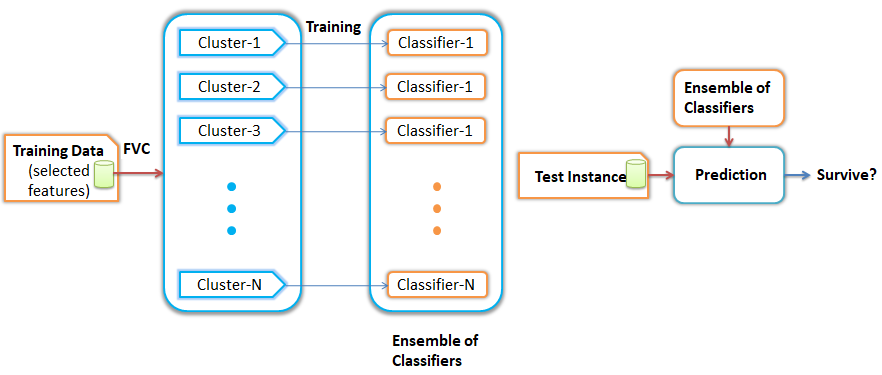
\includegraphics[scale=0.7]{fig/ModelConstructionOverview.png}}
\caption{Model construction overview} \label{fig:ClassificationModelGenerationPhase}
\end{figure}

Figure \ref{fig:ClassificationModelGenerationPhase} presents the high level overview of our model construction methodology. For each dataset, all features are evaluated to understand their importances in the classification task. Several feature ranking algorithms (more details of  these algorithms are in Section \ref{s:feature_ranking_selection}) are applied in this context. Then, based on the ranking scores, a subset of the top-ranked features are selected. Subsequently, training data is clustered using some feature vector compaction (FVC) techniques. Later several classification algorithms are trained on these clusters to form ensemble classifiers.  

\subsection{Feature Ranking and Selection} \label{s:feature_ranking_selection}
\textcolor{blue}{Feature ranking and selection has been successfully applied as an integral step in many machine learning pipeline (recent examples include but not limited to \cite{Zahangir2019, Saifur20181st, Saifur20182nd, Saifur2019})}. Features are evaluated and scored using some ranking algorithms. These evaluators evaluate/rank each of the features in the dataset in the context of the output variable (i.e., the \textit{Class}). Many algorithms are found for ranking features in the literature \cite{Dash:1997, Roberto:2003, Jasmina:2011, Kamkar2015, Baalachandran2015, Zhang2017, Zahangir2019}. \textcolor{blue}{Interestingly some feature ranking algorithms from the Waikato Environment for Knowledge Analysis (popularly known as \textit{Weka}) tool have been found to be useful for medical datasets in \cite{Zahangir2019}. Inspired by \cite{Zahangir2019} we have also used these feature ranking algorithms from \textit{Weka} along with other options.} These are: \textit{InfoGainAttributeEval}, \textit{CorrelationAttributeEval}, \textit{ClassifierAttributeEval} with Random Forest, \textit{ClassifierAttributeEval} with Support Vector Machine (SVM). Once the ranked features are identified, several combinations of features are selected from the feature sets based on the ranking.

\subsection{Feature Vector Compaction}

\begin{figure}[h] 
	\centering 
	\fbox{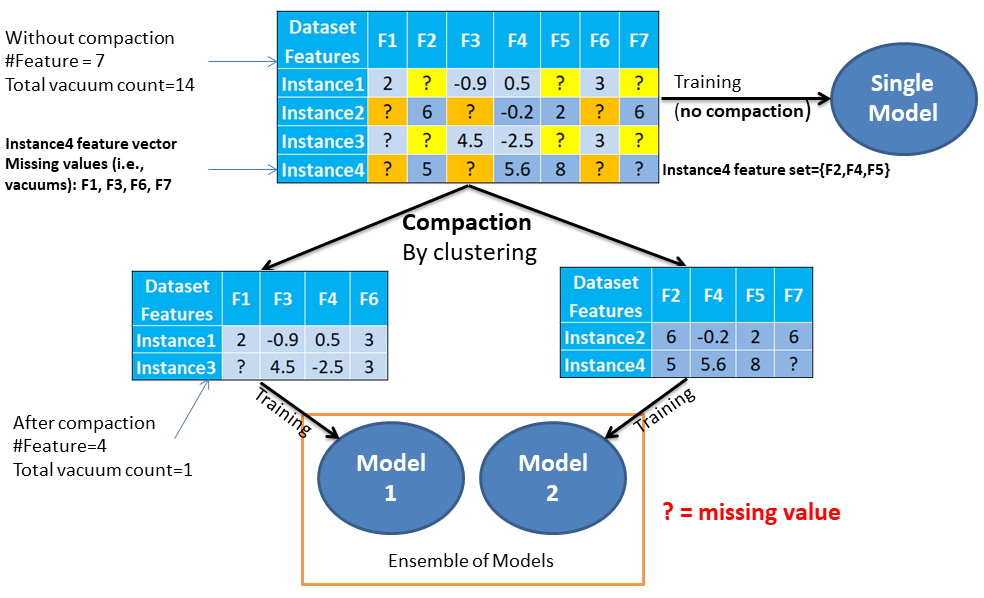
\includegraphics[scale=0.6]{fig/fvc-example-fig.png}}
	\caption{Illustration of Feature Vector Compaction (FVC) technique with example}
	\label{F:fvcwithexample}
\end{figure}

Most of the popular machine learning techniques such as decision tree, SVM and so on, require the feature vector of same features for all instances in order to build predication models. Therefore, for the patient dataset, we need to generate feature vector for each patient by doing the union of the feature sets of all the patients. As a result, empty values are generated for some of the features for some of the patients in the dataset. This sparsity of features not only produces high computational overhead for learning techniques, but also brings noise or redundancy in the data. This issue is increased when we have to work with Big Data, holding thousands of patients information. To deal with the variable feature set we employ Feature Vector Compaction (FVC). It not only minimizes the sparsity of feature vector, but also achieves speedup in learning the prediction and improves the prediction accuracy in most cases. FVC was originally proposed in \cite{mehedy-masud:2017:fvc} by a subset of the authors of this work where some preliminary results were reported. We here exploit FVC and extend its use along several dimensions as will be clear shortly. In general, in FVC technique the patients are grouped (i.e., clustered) according to the similarity of their lab test sets (i.e., feature sets). Figure \ref{F:fvcwithexample} shows the technique with examples.

We also exploit orthogonal clustering (ORCU) which was introduced in \cite{mehedy-masud:2018:frmwrk} by a subset of the authors. Notably, we apply ORCU with some modifications in our research. In orthogonal clustering, dataset is divided into groups in two stages. Every stage has its own clustering technique for grouping data. In the first stage, the dataset is divided by clustering the features (referred to as \textit{Vertical} clustering) and in the second stage, the clustered data from the first stage are further grouped by clustering the subjects (called \textit{Horizontal} clustering).

\begin{algorithm} 
	\caption{ORCU-VH Clustering and Training} 
	\label{a:ORCU-VH}
	{%\footnotesize
		\begin{algorithmic}[1]  
			\REQUIRE {$T$: Raw Training Data}
			\ENSURE { Groups of data $\{D_1, ... D_m\}$ such that 
				$\cup_{i=1}^{m} (D_i) = T$ \\
				$E$: the ensemble classifier,  $E=\{E_1, ... E_m\}$} 
			\STATE $S \leftarrow T$ 
			\STATE $D \leftarrow \phi$
			
			\STATE $S[1], S[2] \leftarrow$ VerticalClustering($S$)//split data using \textit{Vertical} clustering of ORCU					
			
			\FOR {$i \leftarrow$ 1 to 2}
			\STATE $S[i][1], S[i][2] \leftarrow$ HorizontalClustering ($S[i]$) //split data using \textit{Horizontal} clustering of ORCU
			\STATE $D \leftarrow D \cup S[i]$ //generated clusters are put in list
			\ENDFOR
			
			\STATE $m \leftarrow |D|$ //number of data groups
			\FOR {$i \leftarrow$ 1 to $m$}
			\STATE	$E_i \leftarrow $ TrainClassifier($D_i$)
			\ENDFOR    		
		\end{algorithmic}  
	} 
\end{algorithm} 


\begin{algorithm} 
	\caption{ORCU-HV Clustering and Training} 
	\label{a:ORCU-HV}
	{%\footnotesize
		\begin{algorithmic}[1]  
			\REQUIRE {$T$: Raw Training Data}
			\ENSURE { Groups of data $\{D_1, ... D_m\}$ such that 
				$\cup_{i=1}^{m} (D_i) = T$ \\
				$E$: the ensemble classifier,  $E=\{E_1, ... E_m\}$} 
			\STATE $S \leftarrow T$ 
			\STATE $D \leftarrow \phi$
			
			\STATE $S[1], S[2] \leftarrow$ HorizontalClustering($S$)//split data using \textit{Horizontal} clustering of ORCU					
			
			\FOR {$i \leftarrow$ 1 to 2}
			\STATE $S[i][1], S[i][2] \leftarrow$ VerticalClustering($S[i]$) //split data using \textit{Vertical} clustering of ORCU
			\STATE $D \leftarrow D \cup S[i]$ //generated clusters are put in list
			\ENDFOR
			
			\STATE $m \leftarrow |D|$ //number of data groups
			\FOR {$i \leftarrow$ 1 to $m$}
			\STATE	$E_i \leftarrow $ TrainClassifier($D_i$)
			\ENDFOR    		
		\end{algorithmic}  
	} 
\end{algorithm} 

We employ two variations of orthogonal clustering as follows: a) ORCU-VH: in this type, the data is first clustered into two groups by \textit{Vertical} clustering and then the clustered two groups are further divided into four groups using \textit{Horizontal} clustering (please see Algorithm \ref{a:ORCU-VH}); b) ORCU - HV: in this type, the data is clustered in reverse direction of ORCU-VH (i.e., first \textit{Horizontal} clustering followed by \textit{Vertical} clustering) (please see Algorithm \ref{a:ORCU-HV}). 

\subsection{Ensemble Classifiers}
Classifiers are trained on each of the clusters produced at the end of the previous phase. These are used as an ensemble of models $E = {E_1, ...,E_m}$ to classify new patients to predict his mortality. Algorithm 3 (Classify) does the ensemble classification. The input to the algorithm is the instance to be classified, the ensemble of classifiers, and the ensemble approach which is either Vacuum Count (VC) or Common Feature Count (CFC). At first, the test instance is classified by each classifier in the group (the for loop in lines 1-9 does this computation). During this classification process it counts Added Vacuum Count (AVC) \cite{mehedy-masud:2017:fvc} (to be described shortly) or CFC (line 4 and 7). If VC is used then a weighted majority voting is done for the final prediction (lines 10-17). The weight of each model is inversely proportional to the AVC of the test instance and the corresponding dataset of the model. So, lower AVC has higher weight and vice versa. But if CFC is used then the highest CFC value producer (classifier) finally predicts the test instance.  

%But if CFC is used then the prediction of the highest CFC generated ensemble of classifiers is the final prediction (lines 18-21 shows this calculation).       

\begin{algorithm} 
	\caption{Classify} 
	\label{a:Classify}
	{%\footnotesize
		\begin{algorithmic}[1]  
			\REQUIRE {$x$: Instance to classify, $E = \{E_1, ... , E_m \}$: Ensemble of classifiers, $ET = VC$ or $CFC$: Ensemble Technique}
			\ENSURE { $y$: The predicted class} 
			\FOR {$i \leftarrow$ 1 to $m$}
			\STATE $y_i \leftarrow $ Classify($x, E_i$) //Classify
			\IF {$ET = VC$} 	
			\STATE $u_i \leftarrow $ AVC($x, E_i$) //Equation 
			\ref{AVCEquation}
			\ENDIF		
			\IF {$ET = CFC$} 	
			\STATE $u_i \leftarrow $ CFC($x, E_i$) //Equation \ref{CFCEquation}
			\ENDIF		
			\ENDFOR       
			\IF {$ET = VC$}
			\STATE $U \leftarrow \min_{i=1}^m{u_i}$ 
			\FOR {$i \leftarrow$ 1 to $m$}
			\STATE $w_i = U/u_i$       		
			\ENDFOR
			\STATE $W \leftarrow \sum_{i=1}^m{w_i}$ 
			\STATE $y \leftarrow \sum_{i=1}^m{w_i y_i}/W $  			
			\ELSE
			\STATE $i \leftarrow \max_{i=1}^m{u_i}$
			\STATE $y \leftarrow y_i $  
			\ENDIF       
			 
		\end{algorithmic}  
	} 
\end{algorithm} 

\subsubsection{Vacuum counting (VC) method} \label{sec:VCMethod}
Vacuum Count (VC) is the number of vacuums (i.e., empty/missing values) in the instance feature vector. For example, in Figure \ref{F:fvcwithexample}, VC is 4 for \textit{Instance4} (i.e., features F1, F3, F6, and F7 don’t have any value). When two sets of features are merged, the new feature set is created by the union of the two feature sets, which results in generating some vacuums therein. The number of such vacuums is termed as Added vacuums (AVC). For example, suppose a dataset $D$ has feature set $F_D$. If a new instance $d$ is added to $D$, having feature set $F_d$, then the new feature set after merging, $F_{Dnew}$ = $F_D \cup F_d$. Extra vacuums created in the feature vector of $d$ are $|F_{Dnew}|- |F_d|$. So extra vacuums generated in the dataset $D$ are ($|F_{Dnew}| - |F_d|) * n $, where $n$ is the number of instances in $D$ before merging. Therefore, total added vacuums

\begin{equation} \label{AVCEquation}
AVC(D, d) = (|F_{Dnew}| - |F_d|) * (n + 1)
\end{equation}

When an instance of a new patient is considered by the ensemble classification process for prediction, it's missing values are counted with respect to the feature set of each classifier in the ensemble and AVC is computed. 

\subsubsection{Common Feature Counting (CFC) method} \label{sec:CFCMethod}
We propose a new concept called Common Feature Count (CFC) to be used in the ensemble classification process. CFC is defined as follows:

\begin{equation} \label{CFCEquation}
CFC(X,Y_i) = |X \cap Y_i|
\end{equation}

Here, $X$ is the feature set of the corresponding dataset, and $Y_i$ is the (nonempty) feature set of a particular vector $V_i$. For example, if $X$ = {$f_1, f_2, f_3, f_4, f_5$} and $Y_i$ = {$f_2, f_3, f_5, f_6$} then $|X \cap Y_i|$ is 3.

As mentioned earlier, each classifier in the ensemble as well as a test instance has different feature vector. CFC is used to compute the number of common features between a test instance and a classifier in the ensemble. A classification model that has the maximum CFC value is finally used for prediction of this new instance.

%In this methodology, when an instance of new patient is considered into ensemble classification process for prediction, it's CFC is calculated with each cluster for which ensemble model is present. An ensemble model that generates the maximum CFC value is finally used for predicting this new instance.    

%\subsection{Final Model Construction}
%For each dataset, multiple ensemble models are created. In particular, for each dataset, generally 4 separate subset of high ranked features produced by 4 different feature ranking algorithms and four combinations of feature vector grouping, HV, H, VH, V. Thus it leads to form many ensemble models with different combination. We refer to these models using the following form: Model$_{<i>}^{<datasetID-combination>}, 1\leq i \leq 800$. Figure \ref{F:ModelGenOverview} shows how 800 models are generated.

%\begin{figure}[h] 
%	\centering 
%	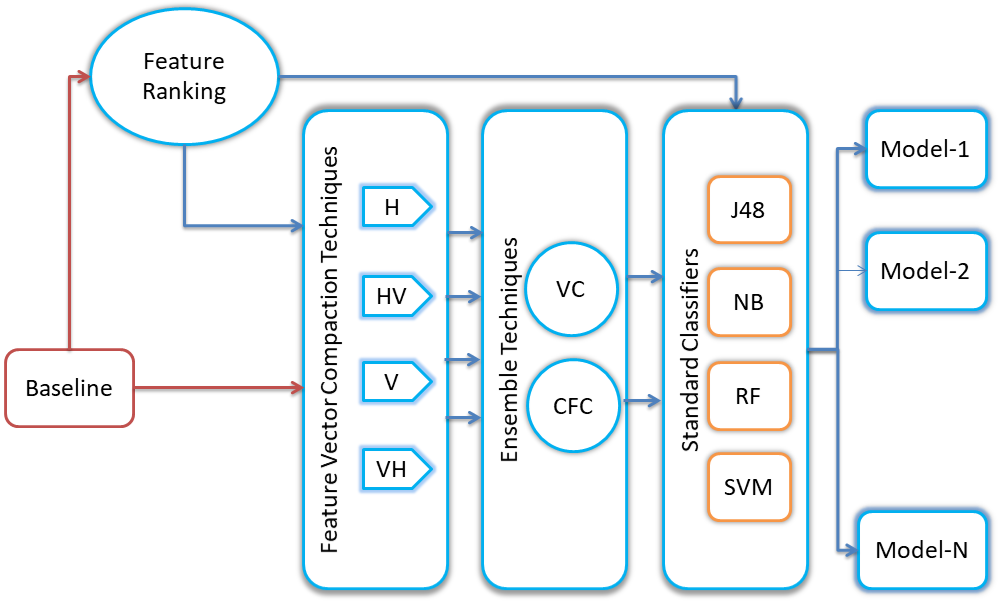
\includegraphics[scale=0.5]{fig/ModelGenOverview.png}
%	\caption{Model Genernation Overview}
%	\label{F:ModelGenOverview}
%\end{figure}

%Additionally, we have constructed the baseline model using all the features, i.e., ignoring the feature ranking exercise; this model is %referred to as Model$_{Base}^{<datasetID>}$. For example, for Adult Binary(F) dataset, for a ranker subset (e.g., R1), for H grouping, for %VC ensemble technique, for J48 classifier the model's name is Model$_\mathrm{i}^\mathrm{AF-R1HVCJ48}$.

	\section{Experiments}\label{s:experiments}
All experiments have been conducted on a CPU with Intel(R) Core(TM) i5-7200U (@ 2.50 GHz) having 8 GB RAM and running Windows 10 operating system. For applying various ranker algorithms, Weka 3.9 \cite{weka} has been used. We evaluate the performance of the models using F-score. F-score is a popular and reliable metric that is widely used in the literature. In fact we report the weighted average F-score in the range of [0,1] ($F_{wa}$) which is defined as follows:

\begin{equation}
F_{WA} = \frac{F_{Alive} * Count_{Alive} +  F_{Dead} * Count_{Dead}}{Count_{Alive} + Count_{Dead}}
\end{equation} 

\subsection{Feature sets for MIMIC-II and MIMIC-III}
\textcolor{blue}{For MIMIC-II datasets, 655 lab tests are identified and these are treated as feature sets for the experiments on MIMIC-II datasets. On the other hand, 570 lab tests are collected and these are used for the experiments on MIMIC-III datasets. The detail list of these lab tests are available int the supplementary file.}
 
\subsection{Notations/Definitions used to represent the results}
The notations defined in Table \ref{t:resultnotations0} and Table \ref{t:resultnotations} are used to present the results.

\begin{table}[h] 
	\centering \caption{Description of some notations used in results} 
	\begin{tabular}{|p{1.25cm}|p{6cm}|p{0.2cm}|p{1.25cm}|p{6cm}|}\hline
		\textbf{Notation} & \textbf{Description} & & \textbf{Notation}  & \textbf{Description} \\\hline
		J48 & J48 classifier & & FVC & Feature Vector Compaction\\\hline
		NB & NaiveBayes classifier & & H & Horizontal clustering \\\hline
		RF & RandomForest classifier & & V & Vertical clustering \\\hline
		SVM & Support vector machine classifier & & HV & First Horizontal and then Vertical clustering \\\hline
		VC & Vacuum Count method & & VH & First Vertical and then Horizontal Clustering \\\hline
		CFC & Common Feature Count method & & & \\\hline  	
	\end{tabular}
	\label{t:resultnotations0}
\end{table}

\begin{table}[h] 
	\centering \caption{Description of ranking notations used in results} 
	\begin{tabular}{|c|c|}\hline
		\textbf{Notation}  & \textbf{Description} \\\hline
		NoR & No Ranking method applied \\\hline
		R1 & $1^{st}$ subset of features by InfoGain ranker. Zero merit valued features are removed. \\\hline
		R1-1 & $2^{nd}$ subset of features by InfoGain ranker. $1/4$ of total ranked features are kept for experiment. \\\hline
		R1-2 & $3^{rd}$ subset of features by InfoGain ranker. $1/2$ of total ranked features are kept for experiment. \\\hline
		R1-3 & $4^{th}$ subset of features by InfoGain ranker. $3/4$ of total ranked features are kept for experiment. \\\hline
		R2 & $1^{st}$ subset of features by Correlation ranker. Zero merit valued features are removed. \\\hline
		R2-1 & $2^{nd}$ subset of features by Correlation ranker. $1/4$ of total ranked features are kept for experiment. \\\hline
		R2-2 & $3^{rd}$ subset of features by Correlation ranker. $1/2$ of total ranked features are kept for experiment. \\\hline
		R2-3 & $4^{th}$ subset of features by InfoGain ranker. $3/4$ of total ranked features are kept for experiment. \\\hline
		R3 & $1^{st}$ subset of features by RandomForest ranker. Zero merit valued features are removed. \\\hline
		R3-1 & $2^{nd}$ subset of features by RandomForest ranker. $1/4$ of total ranked features are kept for experiment. \\\hline
		R3-2 & $3^{rd}$ subset of features by RandomForest ranker. $1/2$ of total ranked features are kept for experiment. \\\hline
		R3-3 & $4^{th}$ subset of features by RandomForest ranker. $3/4$ of total ranked features are kept for experiment. \\\hline
		R4 & $1^{st}$ subset of features by SVM ranker. Zero merit valued features are removed. \\\hline
		R4-1 & $2^{nd}$ subset of features by SVM ranker. $1/4$ of total ranked features are kept for experiment. \\\hline
		R4-2 & $3^{rd}$ subset of features by SVM ranker. $1/2$ of total ranked features are kept for experiment. \\\hline
		R4-3 & $4^{th}$ subset of features by InfoGain ranker. $3/4$ of total ranked features are kept for experiment. \\\hline
	\end{tabular}
	\label{t:resultnotations}
\end{table}

\subsection{Experiments with variations}
For each dataset, multiple ensemble models are created. In particular, for each dataset, 4 separate subsets of high ranked features, produced by 4 different feature ranking algorithms, are combined with four combinations of feature vector grouping, namely, HV (i.e., ORCU-HV), H (i.e., Horizontal), VH (i.e., ORCU-VH), V (i.e., Vertical). Thus a number of models with different combinations are constructed. We refer to these models using the following form: Model$_{<i>}^{<datasetID-combination>}, 1\leq i \leq 572$. Figure \ref{F:ModelGenOverview} shows how these 572 models are generated for each dataset. For example, Model$_\mathrm{i}^\mathrm{AF-R1HVCJ48}$ refers to the model where (a) Adult Binary (F) dataset is used for training \& testing; (b) $1_{st}$ subset of the ranked features (i.e., R1) are used after applying a ranking algorithm; (c) \textit{Horizontal} feature vector compaction has been applied; (d) Vacuum count has been used and (e) J48 has been employed as the classifier algorithm.

\begin{figure}[h] 
	\centering 
	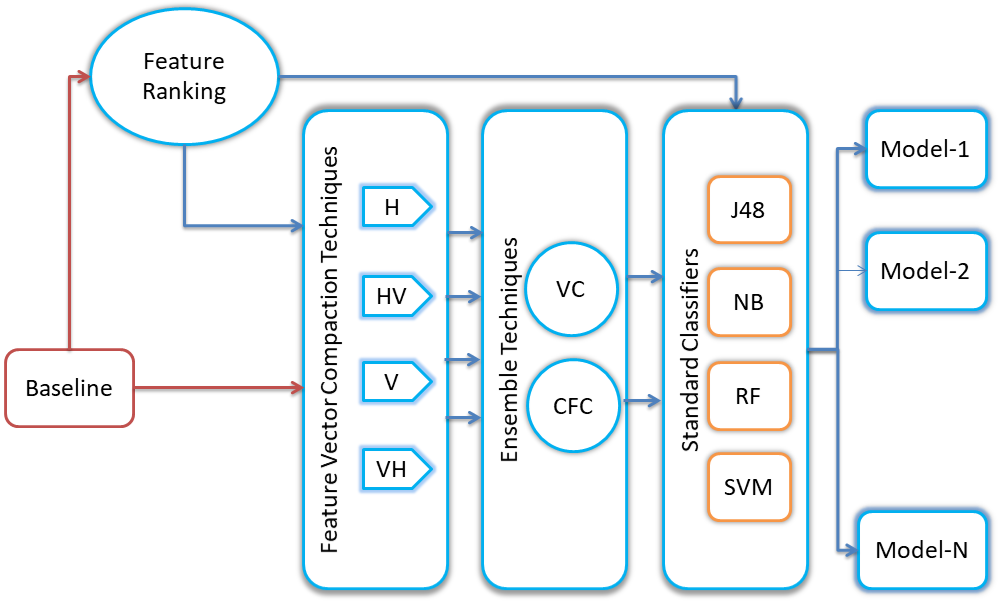
\includegraphics[scale=0.5]{fig/ModelGenOverview.png}
	\caption{Model Generation Overview}
	\label{F:ModelGenOverview}
\end{figure}

So, all considered approaches are listed in Table \ref{t:competingmodels}. Additionally, we have constructed the baseline model using all the features, i.e., ignoring the feature ranking exercise; this model is referred to as Model$_{Base}^{<datasetID>}$.

\begin{table}[h] 
	\centering \caption{Competing approaches} 
	\begin{tabular}{|c|c|c|c|}\hline
		\textbf{Name/Acronym} & \textbf{Reference} & \textbf{Data grouping} & \textbf{Ensambling} \\\hline
		Baseline 1/BL1 & - & - & - \\\hline
		Baseline 2/BL2 & \cite{mehedy-masud:2017:fvc} & FVC & VC \\\hline
		Baseline 3/BL3 & \cite{mehedy-masud:2018:frmwrk} & ORCU-VH & VC \\\hline
		Model$_{<i>}^{<datasetID-combination>}, 1\leq i \leq 3144$ & This study & Horizontal, Vertical, ORCU-VH, ORCU-HV & VC,CFC \\\hline 
	\end{tabular}
	\label{t:competingmodels}
\end{table}
	
	\section{Results}\label{s:results}
A total of 3144 models have been evaluated along with the baselines and some other models reported in the literature for all datasets. The baseline (BL1) output for different datasets are shown in Table \ref{t:baselineoutput}. For all Adult datasets, SVM achieves the highest F-scores, i.e., 80.786, 81.363 and 78.177 for Adult(F), Adult(V) of MIMIC-II and Adult of MIMIC-III datasets respectively. On the other hand, NB achieves the highest scores, i.e., 65.45, 66.083 and 64.569, for Senior (F), Senior (B) of MIMIC-II and Senior of MIMIC-III datasets respectively.  

\begin{table}[h] 
	\centering \caption{Baseline $F_{wa}$ score of the datasets} 
	\begin{tabular}{|c|c|c|c|c|c|c|}\hline	
	Classifier & \multicolumn{4}{|c|}{MIMIC-II} & \multicolumn{2}{|c|}{MIMIC-III} \\\hline
	& Adult(F) & Adult(V) & Senior(F) & Senior(V) & Adult & Senior \\\hline
	J48 & 77.803 & 76.514 & 56.903 & 54.258 & 73.182 & 48.546 \\\hline
	NB & 77.922 & 79.175 & 65.45 & 66.083 & 77.072 & 64.569 \\\hline
	RF & 78.55 & 79.478 & 37.404 & 50.968 & 77.646 & 50.052 \\\hline
	SVM & 80.786 & 81.363 & 64.224 & 61.995 & 78.177 & 57.835 \\\hline
\end{tabular}
\label{t:baselineoutput}
\end{table}

Results of all experiments on these datasets are illustrated in several bar-charts in the following sections (Data corresponding to each of these bar-charts are also available in tabular format in the supplementary file).

\subsection{Results on MIMIC-II Adult Binary (F) dataset}

\begin{figure}[h] 
	\centering
	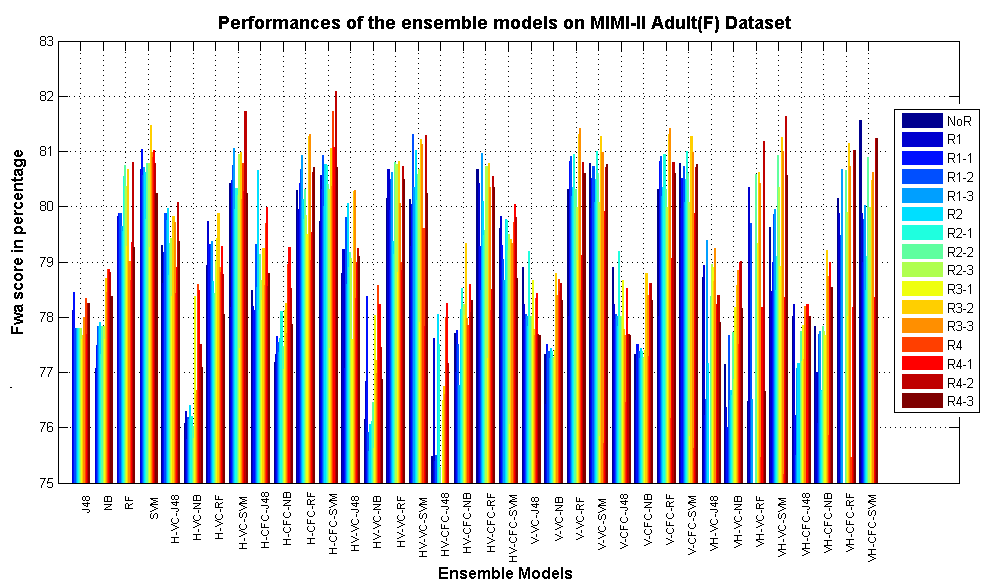
\includegraphics[scale=0.6]{fig/mimic2-adultk1f-full-table.png}
	\caption{$F_{wa}$ score of some experiments on MIMIC-II Adult Binary (F) dataset}
	\label{F:MIMIC2_AdultK1F_Table}
\end{figure}

Figure \ref{F:MIMIC2_AdultK1F_Table} represents the results of the experiments conducted on MIMIC-II Adult Binary (F) dataset. It is evident that after ranking SVM performs well compared to others. For example, when features are ranked by RandomForest and half of the total features are considered, SVM achieves a $F_{wa}$ score of 81.479. When features are compacted after ranking, SVM produces better results as compared to when feature compaction is applied without ranking. For example, SVM produces a $F_{wa}$ score of 81.479 when features are ranked - also by SVM; half of ranked features are selected; and Horizontal feature compaction is applied. The highest $F_{wa}$ score of 82.088 is produced by SVM when features are ranked by SVM; half of the total features are selected; horizontal FVC technique is applied; and finally, CFC is used as the ensemble method. This promising result may be attributed to several reasons, namely, focusing on (eliminating) some highly important and contributing (unimportant) features through ranking and selection, feature grouping and ensemble techniques. When a test instance is classified, it seems logical to use the model having the highest common features between them and thus the CFC approach contributed positively. More details are discussed in Section \ref{s:discussions}. 
 
It is also observed that RF also performs better as compared to J48 or NB for this dataset; in fact J48 and NB do not perform well on this dataset as compared to others. This may be attributed to the issue of how classifiers treat features in prediction. For example, NB treats features as independent, whereas SVM looks at the interactions among these to a certain degree. Naturally, features may be highly correlated for a patient with a disease thereby favouring the latter approach.   

\subsection{Results on MIMIC-II Adult Numeric (V) dataset}

\begin{figure}[h] 
	\centering 
	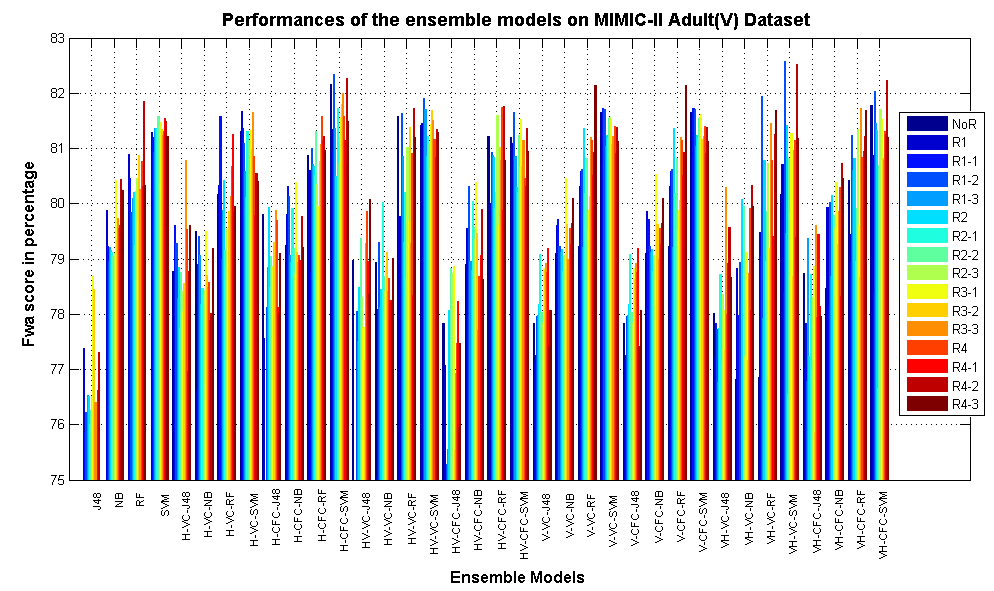
\includegraphics[scale=0.6]{fig/mimic2-adultk1v-full-table.png}
	\caption{$F_{wa}$ score of some experiments on MIMIC-II Adult Number (V) dataset}
	\label{F:MIMIC2_AdultK1V_Table}
\end{figure}

Figure \ref{F:MIMIC2_AdultK1V_Table} shows the results of the experiments conducted on MIMIC-II Adult Numeric (V) dataset. The results on this dataset indicate that SVM alone and its combination with other techniques produce better results. As an example, when features are ranked by SVM, half of the total features are selected, horizontal FVC is used and CFC is employed, then SVM as the classifier achieves a $F_{wa}$ score of 82.26. Changing the Horizontal FVC to Vertical (V) - Horizontal(H) FVC and CFC to VC achieves an even better $F_{wa}$ score of 82.512. But the highest  $F_{wa}$ score of 82.57 for SVM is achieved when features are ranked by Correlation ranker, half of the total features are selected, VH FVC are used and VC is applied as the ensemble technique. It is further observed that J48 and NB are not performing well on this dataset as compared to others using any combination of the techniques although RF observes improved results sometimes with different combinations.    

\subsection{Results on MIMIC-II Senior Binary (F) dataset}

\begin{figure}[h] 
	\centering 
	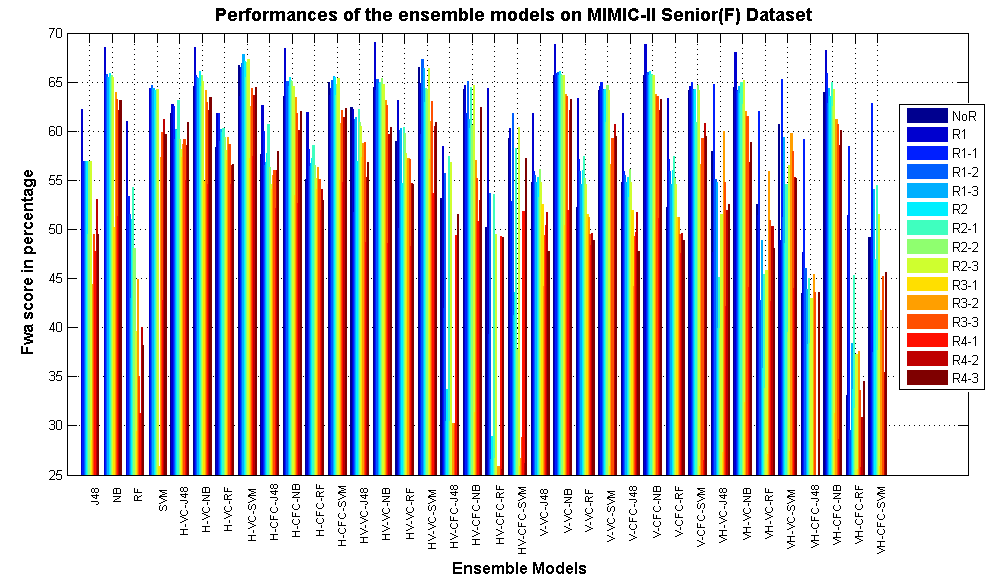
\includegraphics[scale=0.6]{fig/mimic2-seniork1f-full-table.png}
	\caption{$F_{wa}$ score of some experiments on MIMIC-II Senior Binary(F) dataset}
	\label{F:MIMIC2_SeniorK1F_Table}
\end{figure} 

Figure \ref{F:MIMIC2_SeniorK1F_Table} displays the results of the experiments performed on MIMIC-II Senior Binary (F) dataset. Evidently, NB combined with other techniques performs better for this dataset. As an instance, when features are ranked by InfoGain ranker, ${1/4}$th of the total features are selected, NB achieves 68.502 as the $F_{wa}$ score. Just after applying a vector compaction technique following the previous process, the result improves. For example, $F_{wa}$ score of 68.808 is achieved when Vertical(V) vector compaction technique is used with VC ensemble technique. However, the highest $F_{wa}$ score of 69.014 is achieved by NB when features are ranked by InfoGain ranker, ${1/4}$th of the total features are selected, Horizontal(H)-Vertical(V) FVC is used and VC is applied as the ensemble technique. J48 and RF fail to do well on this dataset as compared to others using any combination of the techniques. SVM sometimes has performed better in comparison with these two.    

\subsection{Results on MIMIC-II Senior Numeric (V) dataset}

\begin{figure}[h] 
	\centering 
	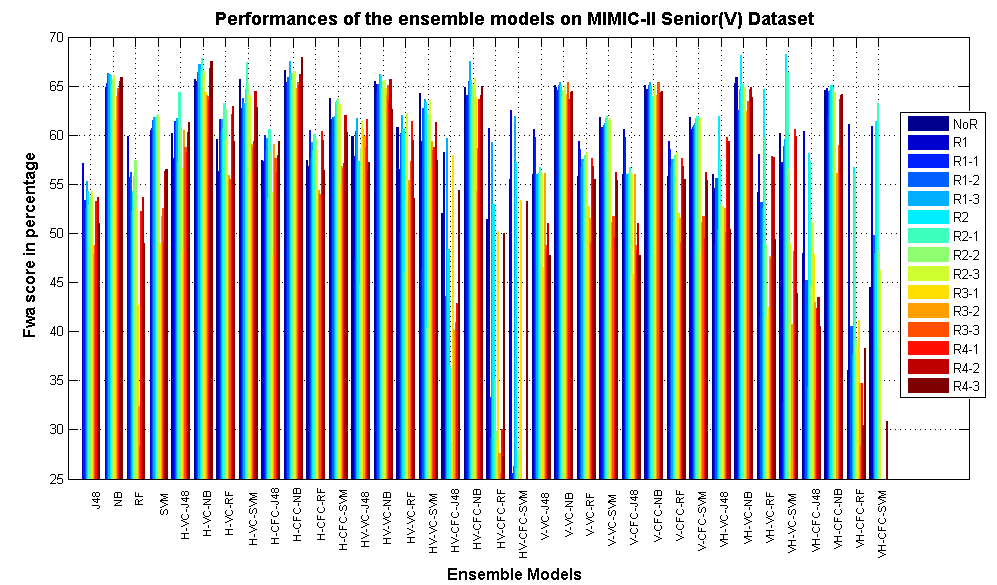
\includegraphics[scale=0.6]{fig/mimic2-seniork1v-full-table.png}
	\caption{$F_{wa}$ score of some experiments on MIMIC-II Senior Numeric (V) dataset}
	\label{F:MIMIC2_SeniorK1V_Table}	
\end{figure} 

Figure \ref{F:MIMIC2_SeniorK1V_Table} shows the results of the experiments conducted on MIMIC-II Senior Numeric (V) dataset. As is evident from the results, NB, combined with other techniques, has achieved better results. For example, when features are ranked by Correlation ranker, half of the total features are selected and Horizontal FVC is used along with VC as the ensemble technique, NB scores 67.806 (as $F_{wa}$ score). However, sometimes SVM combined with other techniques performs better. The highest $F_{wa}$ score of SVM, i.e., 68.215 is achieved when features are ranked by Correlation ranker, ${1/4}$th of the total features are selected, Vertical(V)-Horizontal(V) FVC are used and VC is applied as the ensemble technique. J48 and RF are not performing well on this dataset as compared to others using any combination of the techniques.
 
\subsection{Results on MIMIC-III Adult dataset}
\begin{figure}[h] 
	\centering
	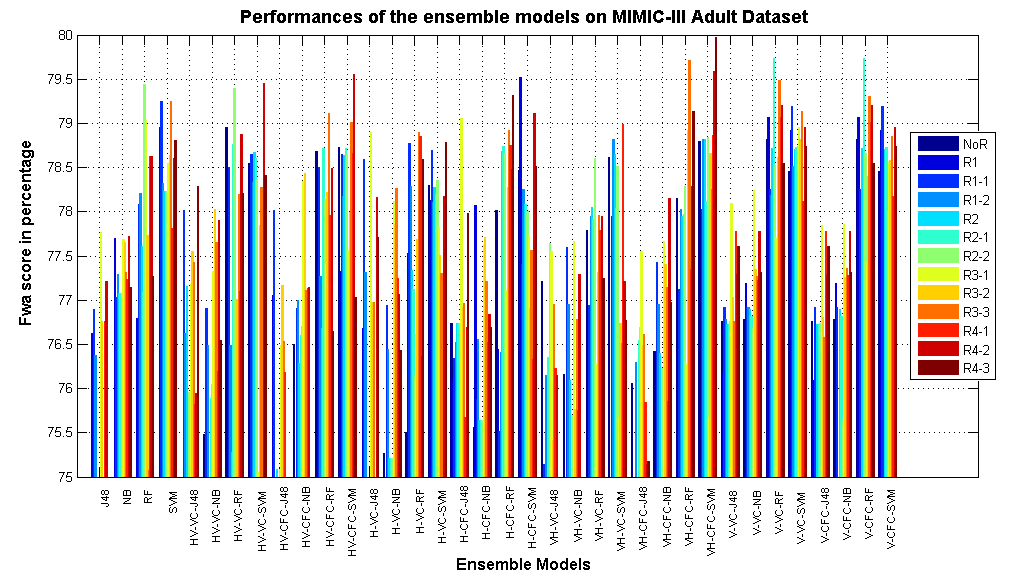
\includegraphics[scale=0.6]{fig/mimic3-adult24hrs-full-table.png}
	\caption{$F_{wa}$ score of some experiments on MIMIC-III Adult dataset}
	\label{F:MIMIC3_Adult24hrs_Table}
\end{figure} 

Figure \ref{F:MIMIC3_Adult24hrs_Table} presents the results of the experiments done on MIMIC-III Adult dataset. The results on this dataset hint that SVM combined with other techniques produces the most competitive results. As an example, when features are ranked by InfoGain ranker, ${3/4}$th of the total features are selected and Horizontal FVC is used along with CFC as the ensemble technique, SVM achieves 79.518 as the $F_{wa}$ score. RF also is observed to have performed well. The highest $F_{wa}$ score of 79.975, produced by SVM is achieved when features are ranked by SVM ranker, ${3/4}$th of the total features are selected, Vertical(V)-Horizontal(V) FVC are used along with CFC ensemble technique. %J48 and NB also perform well on this dataset compared to others using any combination of the techniques.

\subsection{Results on MIMIC-III Senior dataset}

\begin{figure}[h] 
	\centering 
	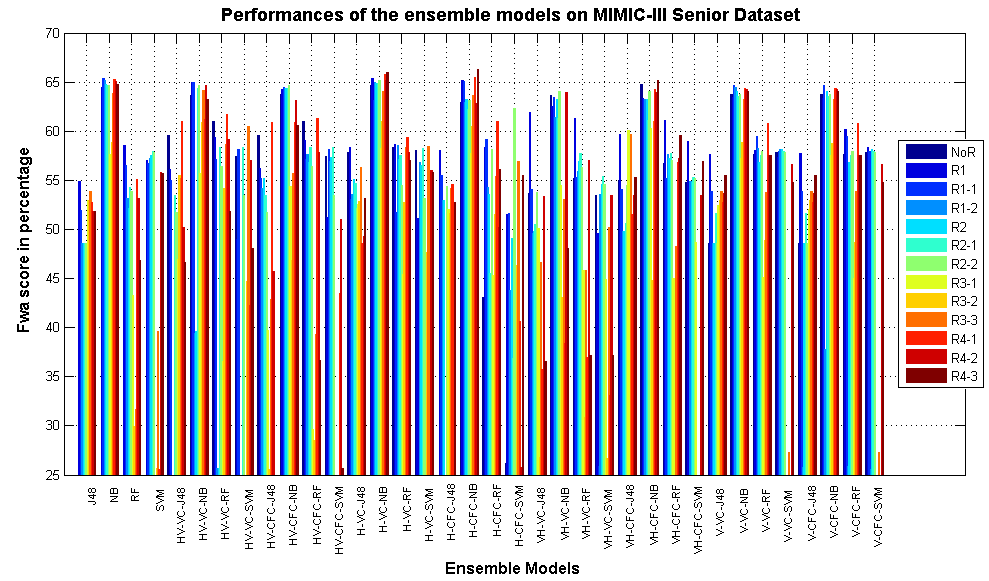
\includegraphics[scale=0.6]{fig/mimic3-senior24hrs-full-table.png}
	\caption{$F_{wa}$ score of some experiments on MIMIC-II Senior dataset}
	\label{F:MIMIC3_Senior24hrs_Table}
\end{figure} 

Figure \ref{F:MIMIC3_Senior24hrs_Table} demonstrates the results of the experiments conducted on MIMIC-III Adult dataset. The results on this dataset show that NB combined with other techniques produces better results. As an example, when features are ranked by SVM ranker,  ${3/4}$th of the total features are selected and Horizontal FVC is used along with VC as the ensemble technique, NB achieves 65.945 as the $F_{wa}$ score. The highest $F_{wa}$ score of 66.333 produced by NB, is achieved when features are ranked by SVM ranker, ${3/4}$th of the total features are selected, Horizontal(V) FVC are used along with CFC as the ensemble technique. Unfortunately other classifiers did not perform well here.

\subsection{Summary comparison with baselines and state of the arts}

\begin{figure}[h] 
	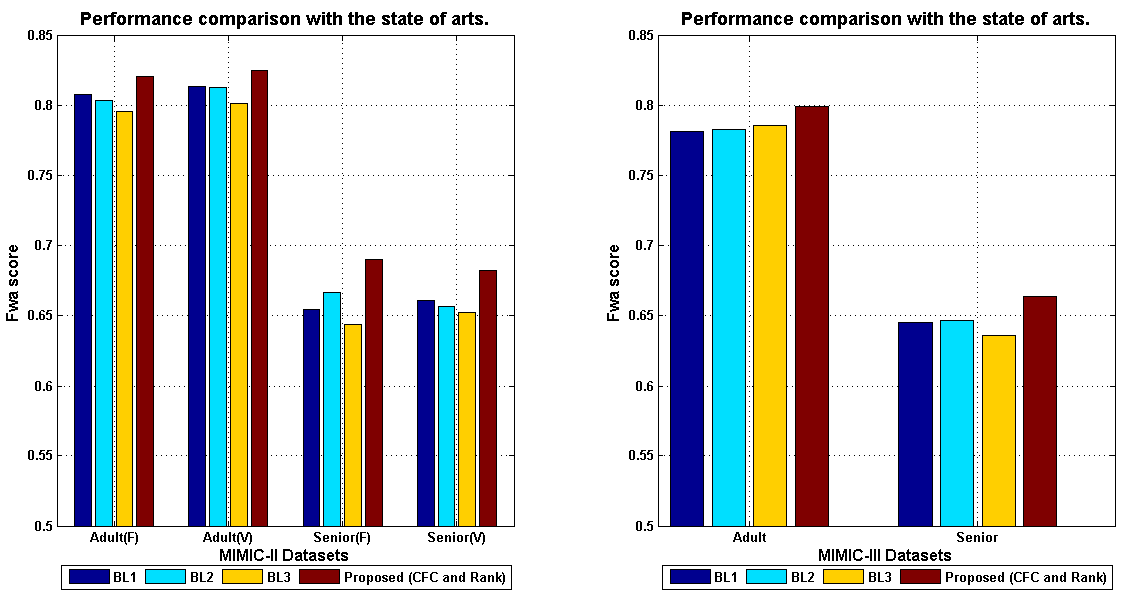
\includegraphics[scale=0.5]{fig/comparison-with-state-of-arts.png}
	\centering \caption{Performance comparison the proposed method with the state of the arts in terms of $F_{wa}$ score. Here BL1 means when no preprocessing technique is applied; BL2 is the technique proposed by the study \cite{mehedy-masud:2017:fvc}; And BL3 is the method introduced in the study \cite{mehedy-masud:2018:frmwrk}. The highest scored ensemble models seen in Figures \ref{F:MIMIC2_AdultK1F_Table} $-$ \ref{F:MIMIC3_Senior24hrs_Table} for each dataset are compared here with the state of the arts.}
	\label{F:comparison_with_state_of_art}
\end{figure}

% Model - i - information
%-----dataset------ Higest - Total
%MIMIC-II-Adult(F) - 187 - 572
%MIMIC-II-Adult(V) - 496 - 572
%MIMIC-II-Senior(F) - 206 - 536
%MIMIC-II-Senior(V) - 498 - 536
%MIMIC-III-Adult - 360 - 464
%MIMIC-III-Senior - 230 - 464
%
%--------------------Total - 3144
%

Figure \ref{F:comparison_with_state_of_art} presents the performance comparison of the proposed technique with the state of the arts, such as, the results produced by the techniques of \cite{mehedy-masud:2017:fvc} (i.e., BL2) and \cite{mehedy-masud:2018:frmwrk} (i.e., BL3) in terms of $F_{wa}$ score. The left panel and the right panel of Figure \ref{F:comparison_with_state_of_art} show the performance of the highest scored model comparing with all previous baselines for each of MIMIC-II and MIMIC-III datasets respectively. For MIMIC-II datasets, Model$_\mathrm{187}^\mathrm{AF-R4-2HCFCSVM}$, Model$_\mathrm{496}^\mathrm{AV-R1-2VHVCSVM}$, Model$_\mathrm{206}^\mathrm{SF-R1HVVCNB}$, and Model$_\mathrm{498}^\mathrm{SV-R2VHVCSVM}$ are the highest scored models for Adult Binary (F), Adult Numeric (V), Senior Binary (F) and Senior Numeric (V) datasets respectively. For MIMIC-III datasets, Model$_\mathrm{360}^\mathrm{AV-R4-3VHCFCSVM}$ and Model$_\mathrm{230}^\mathrm{SV-R4-3HCFCNB}$ are the highest scored models for Adult and Senior datasets respectively. Their $F_{wa}$ scores are compared with all previous baselines in Figure \ref{F:comparison_with_state_of_art}. 

\textcolor{blue}{Table \ref{t:Summary_of_results_with_all_baselines2} presents the results of this study in terms of  Accuracy, Precision, Recall, and F1 score comparing with baselines for each dataset. For each case, it is clearly observed that our model is doing better compared to all the baselines.}

\begin{table}[h] 
	\tiny %\small
	\centering \caption{\textcolor{blue}{Accuracy, Precision, Recall, and F1 score of this study comparing with baselines}} 
	\begin{tabular}{|p{1.5cm}|p{0.6cm}|p{0.6cm}|p{0.6cm}|p{0.6cm}|p{0.6cm}|p{0.6cm}|p{0.6cm}|p{0.6cm}|p{0.6cm}|p{0.6cm}|p{0.6cm}|p{0.6cm}|p{0.6cm}|p{0.6cm}|p{0.6cm}|p{0.6cm}|}\hline	
		& \multicolumn{4}{|c|}{BL1} & \multicolumn{4}{|c|}{BL2} & \multicolumn{4}{|c|}{BL3} & \multicolumn{4}{|c|}{This study} \\\hline	
		DataSet	& Acc. & Pre. & Rec. & F1 & Acc. & Pre. & Rec. & F1 & Acc. & Pre. & Rec. & F1 & Acc. & Pre. & Rec. & F1 \\\hline	
		MIMIC-II Adult (F) & 81.296 & 70.309 & 68.203 & 69.119 & 81.094 & 69.856 & 67.186 & 68.294 & 82.174 & \textbf{72.647} & 62.385 & 64.633 & \textbf{82.512} & 72.442 & \textbf{70.363} & \textbf{71.287} \\\hline 
		MIMIC-II Adult (V) & 81.634 & 71.022 & 69.815 & 70.375 & 81.499 & 70.850 & 69.985 & 70.395 & 82.512 & 73.412 & 63.360 & 65.754 & \textbf{83.255} & \textbf{73.797} & \textbf{70.190} & \textbf{71.672} \\\hline  
		MIMIC-II Senior (F) & 65.681 & 68.189 & 67.689 & 65.635 & 66.683 & 68.228 & 68.200 & 66.683 & 64.679 & 67.263 & 66.725 & 64.621 & \textbf{69.038} & \textbf{68.333} & \textbf{68.276} & \textbf{68.303} \\\hline
		MIMIC-II Senior (V) & 67.184 & 66.831 & 64.684 & 64.705 & 66.232 & 65.387 & 64.428 & 64.557 & 66.483 & 66.108 & 63.846 & 63.783 & \textbf{68.136} & \textbf{67.541} & \textbf{67.716} & \textbf{67.603} \\\hline 
		MIMIC-III Adult & 79.068 & 66.022 & 63.502 & 64.486 & 79.406 & 66.669 & 64.094 & 65.110 & 79.338 & 66.525 & 63.925 & 64.944 & \textbf{80.824} & \textbf{69.268} & \textbf{66.126} & \textbf{67.369} \\\hline
		MIMIC-III Senior & 64.930 & 63.962 & 63.398 & 63.508 & 63.577 & 62.878 & 62.973 & 62.914 & 64.429 & 63.429 & 62.478 & 62.542 & \textbf{66.633} & \textbf{65.774} & \textbf{65.214} & \textbf{65.351} \\\hline  
		
	\end{tabular}
	\label{t:Summary_of_results_with_all_baselines2}
\end{table}

\begin{figure}[h] 
	\centering 
	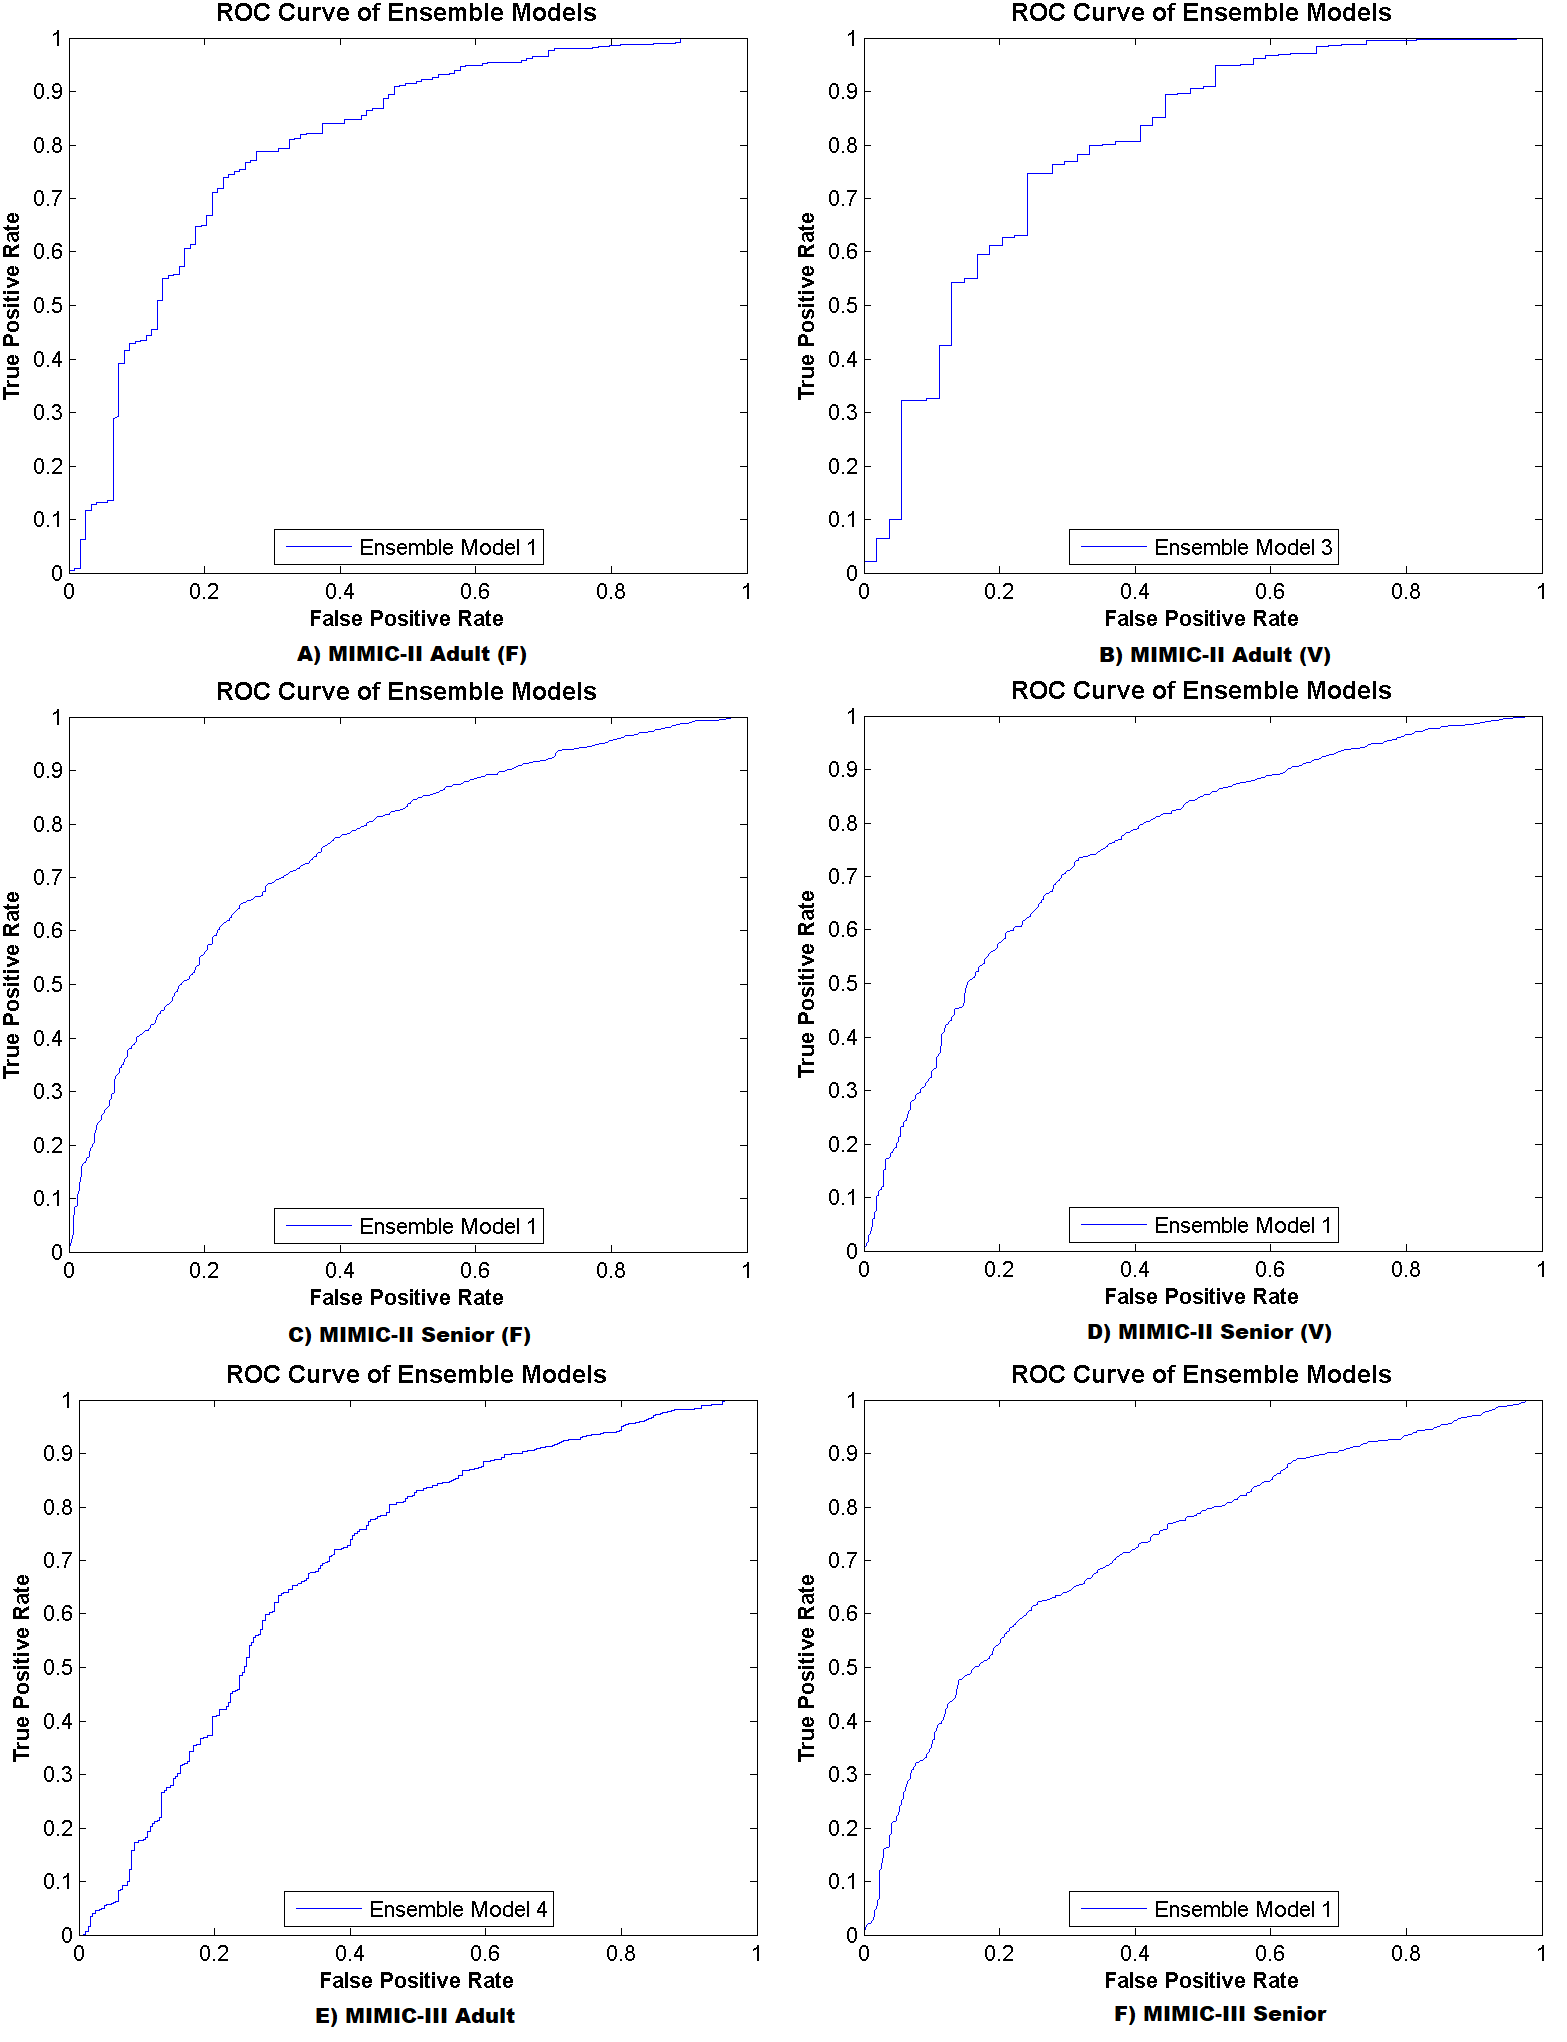
\includegraphics[scale=0.25]{fig/ROC-top.png}
	\caption{ROC Curve of some ensemble models for each dataset}
	\label{F:ROC}
\end{figure} 

In addition to the above results, Figure \ref{F:ROC} presents some ROC curves of some ensemble models which are used in this study for each dataset. Each of these curves is above of the 45-degree diagonal axes and have a tendency towards the top-left corner. These indicate that these models have capability for doing better.      
      
Table \ref{t:Summary_of_results_with_all_baselines} presents the summary of the results of the proposed techniques along with other baselines, i.e, BL1, BL2 and BL3. From these results it is evident that for every dataset, the proposed techniques are producing better results compared to all previous baselines.   

\begin{table}[h] 
	\centering \caption{Summary of the results comparing with baselines in terms of $F_{wa}$ score} 
	\begin{tabular}{|p{0.8cm}|p{1cm}|p{0.6cm}|p{0.8cm}|p{0.6cm}|p{0.8cm}|p{0.6cm}|p{0.8cm}|p{5.0cm}|p{1cm}|p{0.7cm}|}\hline	
		Age group type & Data Type & BL1 & $F_{wa}$ of BL1 & BL2 & $F_{wa}$ of BL2 & BL3 & $F_{wa}$ of BL3 & Proposed (CFC and Rank) & $F_{wa}$ of the proposed & $F_{wa}$ (+/-) over BL3 \\\hline		
		
		\multicolumn{11}{|c|}{\textbf{MIMIC-II}} \\\hline
		Adult & Binary (F) &	SVM	& 80.786 & SVM	& 80.414 &	SVM & 79.618 & First ranking, then H grouping-CFC is used in ensemble (Alg: SVM)	& \textbf{82.088}	& 2.47 \\\hline
		Adult & Numeric (V)	& SVM &	81.363 & SVM & 81.303 & SVM & 80.166 &	First ranking then VH grouping and then VC is used in ensemble (Alg: SVM) &	\textbf{82.57} & 2.404 \\\hline
		Senior & Binary (F) & NB & 65.45 & SVM & 66.671 & NB & 64.41 & First ranking, then HV grouping  and then VC is used in ensemble  (Alg: NB) & \textbf{69.014} &  4.604 \\\hline
		Senior & Numeric (V) & NB & 66.083 & NB & 65.692 & NB & 65.239 & First ranking then VH grouping and then VC is used in ensemble (Alg: SVM) &	\textbf{68.215} & 2.976 \\\hline
		
		\multicolumn{11}{|c|}{\textbf{MIMIC-III}} \\\hline	
		Adult & 24hrs & SVM & 78.177 & SVM & 78.546 & SVM & 78.459 & First ranking then VH grouping and then CFC is used in ensemble (Alg: SVM) &	\textbf{79.975} &  1.516 \\\hline
		Senior & 24hrs & NB & 64.569 & NB & 63.644 & NB & 63.780 & First ranking then H grouping and then CFC is used in ensemble (Alg: NB) &	\textbf{66.333}	& 2.553 \\\hline
		
	\end{tabular}
	\label{t:Summary_of_results_with_all_baselines}
\end{table}



	
	\section{Discussions} \label{s:discussions}
Throughout the extensive experiments conducted, we can notice that feature ranking based FVC techniques along with VC and CFC as the ensemble  technique have performed more accurately. In what follows we discuss these results from different angles and perspectives. 

\subsection{Feature ranking vs. w/o feature ranking}
From Figure \ref{F:MIMIC2_AdultK1F_Table} $-$ \ref{F:MIMIC3_Senior24hrs_Table}, the importance of feature ranking across different combinations of techniques and datasets is already evident. Figure \ref{F:Rank_Comparison_On_MIMICII_MIMICIII} here highlights this information in a more focused and systematic manner as follows.
%For each dataset this comparison is prepared. Figure \ref{F:MIMIC3_Senior24hrs_Table}, \ref{F:MIMIC2_AdultK1F_Table}, \ref{F:MIMIC2_AdultK1V_Table}, \ref{F:MIMIC2_SeniorK1F_Table}, \ref{F:MIMIC2_SeniorK1V_Table} and \ref{F:MIMIC3_Adult24hrs_Table} related to this section contains two information. One is the comparison of the proposed technique with w/o feature ranking approaches. Another one shows how much improvement achieved using proposed technique along with which techniques perform well. For these results, the highest $F_{wa}$ scores are presented to compare.  
The top left panel of Figure \ref{F:Rank_Comparison_On_MIMICII_MIMICIII} clearly reveals that for the MIMIC II Adult Binary (F) dataset when ranking based approaches are used with any FVC technique, the results are superior. It also hints that larger subsets of ranked features perform better. This may be attributed to the fact that among the features with positive (ranking) scores, there are not much difference with respect to importance (which is also evident from their very close importance scores). SVM and RF standout as the main performers as classifiers for doing better. 

\begin{figure}[h] 
	\centering 
	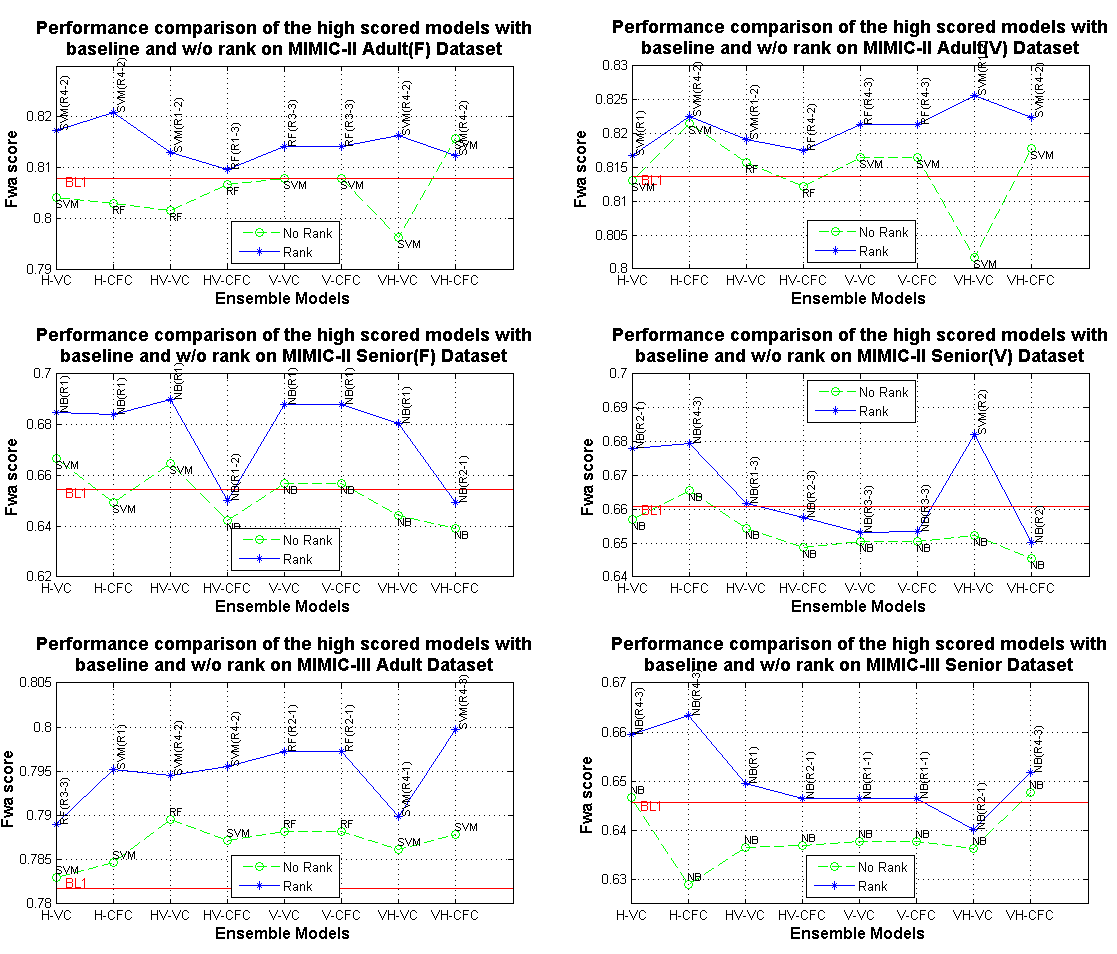
\includegraphics[scale=0.5]{fig/rank-comparison-on-all-datasets.png}
	\caption{Comparison of Feature ranking vs. w/o feature ranking based models in terms of $F_{wa}$ score on MIMIC-II and MIMIC-III datasets}
	\label{F:Rank_Comparison_On_MIMICII_MIMICIII}
\end{figure} 

The top right panel of Figure \ref{F:Rank_Comparison_On_MIMICII_MIMICIII} shows the results on MIMIC-II Adult Numeric (V) dataset. Here as well it is clearly evident that when ranking based approaches are used with any of the FVC techniques, then better results are achieved. Here SVM and RF are the star classifiers. 

The middle left panel of Figure \ref{F:Rank_Comparison_On_MIMICII_MIMICIII} demonstrates the results on MIMIC-II Senior Binary (F) dataset. It also indicates that when ranking based approaches are used with any of the FVC techniques, better results are achieved. Here the improvement is quite remarkable, i.e., 3.5\% improvement over BL1. Here NB is undoubtedly the best performer.

The middle right panel of Figure \ref{F:Rank_Comparison_On_MIMICII_MIMICIII} considers the MIMIC-II Senior Numeric (V) dataset. Here as well we notice the same situation with respect to feature ranking and the improvement is also mentionable, i.e., more than 2\%, over BL1. While NB here stands out with a robust performance overall, the best score is achieved by SVM. 

The bottom left panel of Figure \ref{F:Rank_Comparison_On_MIMICII_MIMICIII} focuses on MIMIC-III Adult dataset. Again the results are consistently in favour of feature ranking. Here NB is the star classifier. Finally, the bottom right panel of Figure \ref{F:Rank_Comparison_On_MIMICII_MIMICIII} focuses on MIMIC-III Senior dataset and the superiority of the combination with feature ranking is clearly evident here as well. For this dataset, NB is again the best performer. Interestingly, NB has performed consistently well for the Senior datasets of MIMIC-II and MIMIC-II, except for the Senior Numeric (V) dataset of MIMIC-II. 

To further check the direct contribution of the feature ranking and selection we have conducted some experiments without feature grouping. The results were better than BL1 in all datasets indicating that feature ranking directly contributes to the robustness of our approach.    

Apart from contributing through ranking and selection of features, feature ranking methodology is believed to have also helped us indirectly as follows. Many records of these datasets contain missing values. These missing values are replaced by the classifiers when the classifiers are trained. These replaced values may not be the true representation. When feature ranking based approach is used, some of these features are removed through the feature selection process thereby helping the classifier by removing `confusing' instances. \textcolor{blue}{For example, Protein S (Functional), Protein C (Functional), Reticulocyte Count (manual or absolute), Quantitative G6PD blood tests are found as low ranked features for Adult group in MIMIC-II and MIMIC-III datasets. Upon examination it has been found that in around 99\% cases the values of Quantitative G6PD, Protein C (Functional), and Protein S (Functional) are missing for Adult group in MIMIC-II datasets and in fact 100\% values of Reticulocyte Count blood test are missing for Adult group in MIMIC-III dataset. Similar situation is also observed for some other attributes/features as well (e.g., HLA-DR (Human Leukocyte Antigen – DR isotype), Heinz Body Prep, Howell-Jolly Bodies, and H/O Smear blood tests are found as low ranked features for Senior group in MIMIC-II datasets as these are missing in around 99\% cases.). Thus the feature ranking \& selection step acted as a filter excluding these 'damaging' features thereby improving the classifier performance.}

\subsection{Feature ranking implications}
In an effort to analyze and understand the implications of feature ranking we have identified the top ten features (based on ranking) of each dataset which are listed in the supplementary document. For every dataset some features, such as, Red blood cell Distribution Width (RDW), Creatinine, Bilirubin, and Urea Nitrogen are found within the top ranked features. From medical perspective these features are very important for a patient and specially when he is at ICU. For example, RDW mainly confirms the presence of anemia. It is also used to evaluate critical conditions, like, cancer, heart disease, liver disorder etc. \textcolor{blue}{In a recent study \cite{Fernandez2018} it has been seen that high RDW is a marker of severity at ICU discharge in the context of in-hospital mortality.} Similarly, high creatinine level indicates kidney disease or a dysfunctional kidney. Thus ranking algorithms have been able to correctly capture these as some of the highly important features among others. Thus, not surprisingly, feature ranking based models have performed better as compared to the baselines.   

We have also performed a statistical correlation analysis on some top ranked features and the patient status (alive/dead). These results are reported in the supplementary file. For each important feature, we estimated the degree of association between that feature and the patient status by fitting a simple linear regression model. Then we assessed the statistical significance of each inferred association using hypothesis testing. We applied the t-test assuming that there is no association which is known as the null hypothesis. The resultant p-value showed us the probability of obtaining a result equal to or ``more extreme" than what was actually observed, when the null hypothesis is true. For all the associations, we obtained p-value 0.0 (rounded to 5 decimal point). So with 99\% confidence we can state these associations to be significant. These results further strengthen our hypothesis that feature ranking and selection was fruitful.        

\subsection{VC vs. CFC}
VC and CFC techniques are used as the ensemble approach to find the right classifier from the ensembles for test instance to do the prediction. The contribution of these techniques depends on the structure of the records of ensemble clusters (through FVC technique) and the structure of the test instance. VC mainly focuses on the missing values present in the ensemble cluster and the test record whereas contrastingly, CFC checks for the common values between the two. Therefore, more missing values guides VC and less missing values aid CFC. 

The results shown in Figure \ref{F:Rank_Comparison_On_MIMICII_MIMICIII} indicate that CFC technique is better for MIMIC-III datasets as compared to VC technique during ensemble classification process. The available features and their values (including missing ones) seen in the datasets of MIMIC-II and MIMIC-III are primarily responsible for these outcomes. For MIMIC-III datasets as compared to MIMIC-II less missing values are found during the ensemble clustering process. Therefore, CFC is performing better for MIMIC-III datasets.             

%The structure of the instances and the availabilities of the feature values in these instances seen in the datasets of MIMIC-II and MIMIC-III are primarily responsible for these outcomes. For MIMIC-III datasets, a test instance gets the closest classifier in terms of CFC value during classification process mostly due to the feature values presentation. Therefore, CFC is performing better for these datasets.            

%\subsubsection{HV vs. H vs. VH vs. V}
%Feature vector compaction techniques depends on primarily vacuum counting between two instances. Therefore, these depend on how much missing values are present in the datasets. From data shown in Figures \ref{F:Rank_Comparison_On_MIMICII_MIMICIII} and results of each dataset of MIMIC-II and MIMIC-III, one thing has been observed that for MIMIC-II numeric datasets (e.g., Adult(V), Senior(V)) VH grouping doing better results. For other datasets these FVC techniques are varied.   
 
\subsection{Results comparing with baselines}
\textcolor{blue}{In the context of mortality or survival prediction of ICU patients, most of the studies \cite{Pirracchio2015, Calvert2016, Bhattacharya2017, Xie2017, Awad2017, Johnson2nd2017, Darabi2018, Davoodi2018, Sadeghi2018, Purushotham2018} found in literature mainly work with vital signs with lab tests to predict the mortality of ICU patients. Some of other works, such as \cite{Ghassemi2015, Marafino2015, Grnarova2016, ZhengpingChe2016}, primarily focus on clinical notes along with these variables. To the best of our knowledge, we found only two works \cite{mehedy-masud:2017:fvc, mehedy-masud:2018:frmwrk} that focus on only lab tests results. Therefore, we compare our results with these studies. Figure \ref{F:comparison_with_state_of_art}, Table \ref{t:Summary_of_results_with_all_baselines2}, and Table \ref{t:Summary_of_results_with_all_baselines} present our results comparing with these relevant studies and show the improved performances in all matrics.}  

\textcolor{blue}{Johnson \textit{et al.} conducted a study to reproduce the cohorts used in some studies in the context of performance comparison of the mortality prediction models for the ICU patients using MIMIC datasets \cite{Johnson2nd2017}. They stated that the accurate reproduction of the studies found in the literature can't be guaranteed in this context but their results may be compared by following consistent model design and methodology. In our study, we have followed this principal and present our results comparing with all baselines from the relevant studies \cite{mehedy-masud:2017:fvc, mehedy-masud:2018:frmwrk}.}

\textcolor{blue}{Most of the studies found in the literature either work on MIMIC-II dataset or MIMIC-III dataset as reported in the comparison of benchmark works in a recent study \cite{Purushotham2018}. Purushotham \textit{et al.} performed this study \cite{Purushotham2018} to present benchmark results in the context of some clinical prediction tasks (such as mortality prediction, LoS prediction, and ICD-9 code group prediction). They conducted experiments on MIMIC-III database and formed three sets of features as follows. Feature set A contains 17 features (pre-processed) used in the calculation of the SAPS-II score. Feature set B contains 20 features corresponding to 17 pre-processed features used in Feature set A. Here raw values of the features are used instead of pre-processed ones. Feature set C contains 136 features with raw values. In this set, 20 features of feature set B are available. In these feature sets, vital signs are primary features. On the other hand, our study mainly focus on lab test records for MIMIC-II and MIMIC-III datasets. We have conducted our experiments on a large set of lab tests, namely, 655 lab tests from MIMIC-II datasets and 570 lab tests from MIMIC-III datasets.}  
 
\subsection{About feature sets used here}
\textcolor{blue}{As has been discussed while reviewing the literature we could not find any research work that only considers lab test results for mortality prediction. Here we bring about that discussion in a more focused manner. The works of Calvert \textit{et al.} \cite{Calvert2016}, Johnson \textit{et al.} \cite{Johnson2nd2017}, and Purushotham \textit{et al.} \cite{Purushotham2018} exploited some lab test results (along with other features) in their models. All those lab test results have been included in our feature set. Caicedo-Torres and Gutierrez also used few lab tests in their study \cite{Torres2019}. All these lab tests are included in our feature sets.} 

	\section{Conclusion} \label{s:conclusion}
ICU patients must be closely monitored by health care providers. Early mortality prediction can help them to take proper and timely actions for these patients. The existing researches are mostly based on the vital signs. Very few studies are available in the literature on mortality prediction using lab tests data. We have proposed feature ranking based methods hybridized with other feature vector compaction (FVC) processes utilizing common feature counting (CFC) and vacuum count (VC) ensemble techniques to predict mortality more accurately using the lab tests data. 
      
To advance the current state of the art, this study proposes the feature ranking based approaches, the modification of FVC techniques and CFC as an ensemble technique. From the results of extensive experiments, it has been seen that the proposed technique outperforms other models for predicting mortality using lab test data. 

The study additionally shows how CFC can contribute in improving the performance of the model. In addition to that, it demonstrates the impact of Vertical(V)-Horizontal (H) FVC technique along with Vacuum Count (VC) for better performance. Moreover, this work also compares the performance of some standard classifier algorithms in this context, such as, J48 classifier, NaiveBayes (NB) classifier, RandomForest (RF) classifier and Support Vector Machine (SVM).           
  
In future, we plan to integrate background knowledge on data into our approach. Additionally, missing value replacement using some other methods will be examined and evaluated. The issue of longitudinal feature in the lab tests data will be addressed. For the real world works at ICU, the lab test data will be merged with vital signs to predict mortality rate more accurately as a whole. Currently, some subsets of features from the ranked features are considered for the model; more fine tuning in the feature selection processes may lead us to even better performance. Finally, these proposed models will be applied to other areas of clinical decision support systems where the data exhibits similar properties.
	
	%% The Appendices part is started with the command \appendix;
	%% appendix sections are then done as normal sections
	%% \appendix
	
	%\appendix
%	\section{Orthogonal Clustering} \label{sec:appendices}
%	Appendix one text goes here.
%	
	% you can choose not to have a title for an appendix
	% if you want by leaving the argument blank
%	\section{Appendix two}
%	Appendix two text goes here.
	
	\section*{Supplementary materials:}
	\textcolor{blue}{\textit{ecrc-paper-Suppl.pdf} file contains all supplementary materials.}
	
	\section*{Acknowledgements}
	The first author is supported by an ICT Fellowship administered by ICT Division, Government of the People's Republic of Bangladesh, website: \url{http://www.ictd.gov.bd/}. \textcolor{blue}{This work was also supported in part by ADEK Award for Research Excellence (AARE) Award
	No: AARE17-182}
	

	%% \section{}
	%% \label{}
	
	%% References
	%%
	%% Following citation commands can be used in the body text:
	%% Usage of \cite is as follows:
	%%   \cite{key}         ==>>  [#]
	%%   \cite[chap. 2]{key} ==>> [#, chap. 2]
	%%
	
	%% References with BibTeX database:
	
	%%%%%%%%%%%%%%%%%%%%%%%
	%% Elsevier bibliography styles
	%%%%%%%%%%%%%%%%%%%%%%%
	%% To change the style, put a % in front of the second line of the current style and
	%% remove the % from the second line of the style you would like to use.
	%%%%%%%%%%%%%%%%%%%%%%%
	
	%% Numbered
	%\bibliographystyle{model1-num-names}
	
	%% Numbered without titles
	%\bibliographystyle{model1a-num-names}
	
	%% Harvard
	%\bibliographystyle{model2-names.bst}\biboptions{authoryear}
	
	%% Vancouver numbered
	%\usepackage{numcompress}\bibliographystyle{model3-num-names}
	
	%% Vancouver name/year
	%\usepackage{numcompress}\bibliographystyle{model4-names}\biboptions{authoryear}
	
	%% APA style
	%\bibliographystyle{model5-names}\biboptions{authoryear}
	
	%% AMA style
	%\usepackage{numcompress}\bibliographystyle{model6-num-names}
	
	%% `Elsevier LaTeX' style
	\bibliographystyle{elsarticle-num}
	%%%%%%%%%%%%%%%%%%%%%%%
	\bibliography{mybibfile}
	
	%% Authors are advised to use a BibTeX database file for their reference list.
	%% The provided style file elsarticle-num.bst formats references in the required Procedia style
	
	%% For references without a BibTeX database:
	
	% \begin{thebibliography}{00}
	
	%% \bibitem must have the following form:
	%%   \bibitem{key}...
	%%
	
	% \bibitem{}
	
	% \end{thebibliography}
	
	%\input{experimenttables}
	
\end{document}

%%
%% End of file `ecrc-template.tex'. 